% main.tex: the four-page workshop paper. IEEEtran in conference mode, which the call allows (docs/venue.md, section 3).
%
% Rules of this folder (README.md has the detail):
%   1. No result is typed into a section. Results are macros from generated/numbers.tex, protocol constants are
%      macros from generated/protocol.tex, and settings copied by hand are macros in numbers_by_hand.tex.
%      A quantity that is already measured, or quoted from a cited paper, is typed with "% src: ..." on its line.
%   2. Double blind: no names, institutions, usernames, repository or hub names, home paths, thanks.
%   3. python3 check_paper.py passes before every upload, and with --final before the submission.
%
% Built with tectonic 0.17.0 since 2026-10-08 (README.md, "Building"). Standard packages only.

\documentclass[conference]{IEEEtran}

% Fonts. IEEEtran asks for Times by its old name (ptm), which exists for pdfLaTeX only. Under XeTeX, which tectonic
% runs, that name is undefined: every shape fell back to one upright default font, so nothing in the paper was bold,
% italic or in small capitals (the build log had about 40 "Font shape TU/ptm/... undefined"; seen by the author in
% the built PDF on 2026-10-09). TeX Gyre Termes, Heros and Cursor are the free equivalents of Times, Helvetica and
% Courier and have every shape. With pdfLaTeX (Overleaf's default) the class's own fonts are used as before.
\usepackage{iftex}
\ifPDFTeX\else
  \usepackage{fontspec}
  % named by file, so that the fonts come from the TeX distribution and not from whatever the computer has installed
  \setmainfont{texgyretermes}[Extension=.otf, UprightFont=*-regular, BoldFont=*-bold, ItalicFont=*-italic, BoldItalicFont=*-bolditalic]
  \setsansfont{texgyreheros}[Extension=.otf, UprightFont=*-regular, BoldFont=*-bold, ItalicFont=*-italic, BoldItalicFont=*-bolditalic]
  \setmonofont{texgyrecursor}[Extension=.otf, UprightFont=*-regular, BoldFont=*-bold, ItalicFont=*-italic, BoldItalicFont=*-bolditalic]
\fi

\usepackage{cite}
\usepackage{amsmath}
\usepackage{graphicx}
\usepackage{booktabs}
\usepackage{xspace}
\usepackage[hidelinks]{hyperref}
\usepackage{xurl} % lets a long link in the references break at any character: one ran into the next column
\hypersetup{pdfauthor={Anonymous}, pdftitle={}, pdfsubject={}, pdfkeywords={}}

% --- Draft marks ------------------------------------------------------------------------------------------------------
% \pending{...} printed a bold tag in front of a sentence whose wording still depended on a result. Every IF block was
% settled from the counted report on 2026-10-08 and no tag is left; check_paper.py --final fails if one comes back or
% if the switch below is turned on again.
\newif\ifdraftmarks
\draftmarksfalse
\newcommand{\pending}[1]{\ifdraftmarks\textbf{[#1]}\ \fi}

% --- Figures ----------------------------------------------------------------------------------------------------------
% \figureorbox{file}{height}{what the figure will show}: the figure if its file exists, a framed box of the planned
% height if not, so the page budget holds before the figures are drawn. File names: letters, digits, hyphens only.
\newcommand{\figureorbox}[3]{%
  \IfFileExists{#1}{\includegraphics[width=\columnwidth]{#1}}{%
    \fbox{\parbox[c][#2][c]{0.94\columnwidth}{\centering\footnotesize\textbf{Figure not drawn yet.} #3}}}}

% --- Numbers ----------------------------------------------------------------------------------------------------------
% A radius is a block fit (\radiusClusteredThreshold, \radiusReplay) unless the text says "pooled" (\radiusClustered,
% \radiusSpread): README.md, "Which radius is which".
% GENERATED FILE: do not edit by hand. Written by paper/make_numbers_stub.py from config/protocol.toml.
% protocol version: 1.0
% protocol status: frozen
% While the status is not frozen these values may still change: run the script again after any change.

\newcommand{\protocolVersion}{1.0\xspace} % version of the protocol the paper describes | src: config/protocol.toml, protocol.version
\newcommand{\gridCols}{5\xspace} % columns of the grid | src: config/protocol.toml, table.cols
\newcommand{\gridRows}{3\xspace} % rows of the grid | src: config/protocol.toml, table.rows
\newcommand{\cellSize}{50\xspace} % side of a grid cell, mm | src: config/protocol.toml, table.cell_mm
\newcommand{\cubeEdge}{30\xspace} % edge of the cube, mm | src: config/protocol.toml, table.cube_edge_mm
\newcommand{\nCellsHeldOut}{4\xspace} % cells in which no demonstration starts | src: config/protocol.toml, table.held_out_cells (count)
\newcommand{\heldOutCells}{A1, B2, D2 and E3\xspace} % their names, in words | src: config/protocol.toml, table.held_out_cells (names)
\newcommand{\nCellsTrained}{11\xspace} % cells in which demonstrations start | src: config/protocol.toml, table.cols x table.rows - held-out cells
\newcommand{\testMargin}{5\xspace} % test placements stay this far inside the grid's edge, mm | src: config/protocol.toml, table.test_region_margin_mm
\newcommand{\placementTolerance}{2\xspace} % a reset is accepted within this distance of its target, mm | src: config/protocol.toml, placement.tolerance_mm
\newcommand{\levelMatch}{0.5\xspace} % a requested distance is met within this, mm | src: config/protocol.toml, placement.level_match_mm
\newcommand{\nDemosPerCell}{5\xspace} % demonstrations per trained cell, in both layouts | src: config/protocol.toml, datasets.episodes_per_cell
\newcommand{\nDemos}{55\xspace} % demonstrations in each dataset: the budget | src: config/protocol.toml, trained cells x datasets.episodes_per_cell
\newcommand{\nPointsClustered}{11\xspace} % distinct start points of the clustered layout | src: config/protocol.toml, trained cells (one point each)
\newcommand{\nPointsSpread}{55\xspace} % distinct starts of the spread layout | src: config/protocol.toml, trained cells x datasets.episodes_per_cell (all distinct)
\newcommand{\spreadMinSpacing}{12\xspace} % smallest planned distance between two spread starts, mm | src: config/protocol.toml, datasets.spread_min_spacing_mm
\newcommand{\clusteredMaxDistInCell}{35\xspace} % farthest point of a trained cell from its centre, mm | src: config/protocol.toml, table.cell_mm / sqrt(2), rounded
\newcommand{\nSittings}{4\xspace} % recording sittings, alternating the two layouts | src: config/protocol.toml, datasets.sittings (count)
\newcommand{\trainSteps}{80,000\xspace} % training step at which both policies are evaluated | src: config/protocol.toml, training.evaluation_checkpoint
\newcommand{\trainStepsFallback}{40,000\xspace} % smallest step the fallback rule allows | src: config/protocol.toml, training.fallback_min_checkpoint
\newcommand{\stepInitial}{10\xspace} % staircase step until the first reversal, mm | src: config/protocol.toml, staircase.step_initial_mm
\newcommand{\stepFinal}{5\xspace} % staircase step after the first reversal, mm | src: config/protocol.toml, staircase.step_final_mm
\newcommand{\plannedReplay}{22\xspace} % replay trials planned | src: config/protocol.toml, blocks.T1b (anchors + staircases)
\newcommand{\plannedClustered}{34\xspace} % clustered-policy threshold trials planned | src: config/protocol.toml, blocks.T1a (anchors + staircases)
\newcommand{\plannedWorkspace}{52\xspace} % workspace-test trials planned | src: config/protocol.toml, blocks.T2.pairs x conditions
\newcommand{\plannedSpread}{24\xspace} % spread-policy threshold trials planned | src: config/protocol.toml, blocks.T3 (anchors + staircases)
\newcommand{\plannedTotal}{132\xspace} % scored trials planned in all | src: config/protocol.toml, sum of the four blocks
\newcommand{\nPairsPlanned}{26\xspace} % placements planned for the workspace test | src: config/protocol.toml, blocks.T2.pairs
\newcommand{\nPairsTrainedPlanned}{13\xspace} % of them, placements drawn over the trained cells | src: config/protocol.toml, blocks.T2.regions[trained_cells].pairs
\newcommand{\nPairsHeldOutPlanned}{13\xspace} % of them, placements drawn over the held-out cells | src: config/protocol.toml, blocks.T2.regions[held_out_cells].pairs
\newcommand{\anchorsZeroReplay}{4\xspace} % replay trials planned at d = 0 | src: config/protocol.toml, blocks.T1b.anchors_zero
\newcommand{\anchorsZeroClustered}{6\xspace} % clustered-policy trials planned at d = 0 | src: config/protocol.toml, blocks.T1a.anchors_zero
\newcommand{\anchorsFarClustered}{4\xspace} % clustered-policy trials planned at the far distance | src: config/protocol.toml, blocks.T1a.anchors_far
\newcommand{\anchorsZeroSpread}{4\xspace} % spread-policy trials planned at d = 0 | src: config/protocol.toml, blocks.T3.anchors_zero
\newcommand{\farLevel}{40\xspace} % the far anchor distance, mm | src: config/protocol.toml, blocks.T1a.far_level_mm
\newcommand{\stairTrialsReplay}{9\xspace} % trials in each of the replay's two staircases | src: config/protocol.toml, blocks.T1b.staircases[].trials
\newcommand{\stairTrialsClustered}{12\xspace} % trials in each of the clustered policy's two staircases | src: config/protocol.toml, blocks.T1a.staircases[].trials
\newcommand{\stairTrialsSpread}{10\xspace} % trials in each of the spread policy's two staircases | src: config/protocol.toml, blocks.T3.staircases[].trials
\newcommand{\stairStartNearReplay}{5\xspace} % start of the replay's near staircase, mm | src: config/protocol.toml, blocks.T1b.staircases[up].start_level_mm
\newcommand{\stairStartFarReplay}{25\xspace} % start of the replay's far staircase, mm | src: config/protocol.toml, blocks.T1b.staircases[down].start_level_mm
\newcommand{\stairStartNearClustered}{10\xspace} % start of the clustered policy's near staircase, mm | src: config/protocol.toml, blocks.T1a.staircases[up].start_level_mm
\newcommand{\stairStartFarClustered}{40\xspace} % start of the clustered policy's far staircase, mm | src: config/protocol.toml, blocks.T1a.staircases[down].start_level_mm
\newcommand{\stairStartNearSpread}{5\xspace} % start of the spread policy's near staircase, mm | src: config/protocol.toml, blocks.T3.staircases[up].start_level_mm
\newcommand{\stairStartFarSpread}{25\xspace} % start of the spread policy's far staircase, mm | src: config/protocol.toml, blocks.T3.staircases[down].start_level_mm
\newcommand{\maxLevelReplay}{50\xspace} % largest distance a replay staircase may request, mm | src: config/protocol.toml, blocks.T1b.max_level_mm
\newcommand{\maxLevelClustered}{50\xspace} % largest distance a clustered-policy staircase may request, mm | src: config/protocol.toml, blocks.T1a.max_level_mm
\newcommand{\maxLevelSpread}{50\xspace} % largest distance a spread-policy staircase may request, mm | src: config/protocol.toml, blocks.T3.max_level_mm
\newcommand{\gridRadiusMax}{80\xspace} % upper end of the prior on the tolerance radius, mm | src: config/protocol.toml, analysis.r50_grid_mm.max
\newcommand{\gridWidthMin}{0.5\xspace} % lower end of the prior on the curve's width, mm | src: config/protocol.toml, analysis.width_grid_mm.min
\newcommand{\gridWidthMax}{20\xspace} % upper end of the prior on the curve's width, mm | src: config/protocol.toml, analysis.width_grid_mm.max
\newcommand{\lapseValues}{0, 0.02, 0.05, 0.10\xspace} % the lapse rates the model weighs, for use inside math braces | src: config/protocol.toml, analysis.lapse_values
\newcommand{\lapseValuesWide}{0, 0.02, 0.05, 0.10, 0.20, 0.35, 0.50\xspace} % the longer list of lapse rates of the plateau check, for use inside math braces | src: config/protocol.toml, analysis.lapse_values_sensitivity
\newcommand{\plateauShiftLimit}{5\xspace} % how far the radii of a fit and of its plateau check may lie apart before the plateau is in doubt, mm | src: config/protocol.toml, analysis.sensitivity_limit_mm
\newcommand{\floorValues}{0, 0.05, 0.10\xspace} % the floors the model weighs (the chance of a success far from every demonstration), for use inside math braces | src: config/protocol.toml, analysis.floor_values
\newcommand{\nReplayDemosPlanned}{11\xspace} % demonstrations the replay block plays back, each from another cell | src: config/protocol.toml, blocks.T1b.replay_demos
\newcommand{\handoffTolerance}{8\xspace} % how far a policy's first command may be from the arm's pose, degrees per joint | src: config/protocol.toml, execution.handoff_tolerance_deg
\newcommand{\handoffToleranceReplay}{5\xspace} % the same for a replay, degrees per joint | src: config/protocol.toml, execution.replay_handoff_tolerance_deg
\newcommand{\viewCreptLimit}{1\xspace} % no attempt once the front camera's picture stands this far from where its session solved the conversion, mm | src: config/protocol.toml, execution.view_crept_limit_mm
\newcommand{\intervalLevel}{95\xspace} % level of every reported interval, percent | src: config/protocol.toml, analysis.interval_level x 100

% GENERATED FILE: do not edit by hand. Written by paper/make_numbers_stub.py.
% The results of the experiment, one macro each. generated/MACROS.md says what each holds.
% A macro that prints a bold ?? has no value yet: 17 of 217 are placeholders.
% After a macro write a space, a unit joined by a tie (~mm, ~\%), punctuation, or {}. Never \, or ].

% --- sim: Simulation of the procedure, before the protocol is frozen
%     produced from: the procedure simulation (analysis/simulation/procedure.md); no trials
\newcommand{\simTruthRadius}{20.0\xspace} % tolerance radius assumed true in the reported simulation, mm | src: analysis/simulation/procedure.csv, the case fixed before the data (simulated, not measured)
\newcommand{\simTruthWidth}{3.0\xspace} % width of the success curve assumed true in the reported simulation, mm | src: analysis/simulation/procedure.csv, the case fixed before the data (simulated, not measured)
\newcommand{\simReplications}{300\xspace} % number of simulated blocks behind each simulation figure | src: analysis/simulation/procedure.csv, the case fixed before the data (simulated, not measured)
\newcommand{\simBias}{\ensuremath{-}0.2\xspace} % mean of (estimated radius - true radius) for the clustered policy's block as planned, mm | src: analysis/simulation/procedure.csv, the case fixed before the data (simulated, not measured)
\newcommand{\simRmse}{1.6\xspace} % root-mean-square error of the estimated radius for that block, mm | src: analysis/simulation/procedure.csv, the case fixed before the data (simulated, not measured)
\newcommand{\simIntervalWidth}{7.8\xspace} % mean width of the 95 % interval of the radius for that block, mm | src: analysis/simulation/procedure.csv, the case fixed before the data (simulated, not measured)
\newcommand{\simCoverage}{97\xspace} % share of simulated blocks whose 95 % interval held the true radius, percent | src: analysis/simulation/procedure.csv, the case fixed before the data (simulated, not measured)
\newcommand{\simRmseConstant}{2.3\xspace} % the same error with the block's trials at fixed, equally spaced distances, mm | src: analysis/simulation/procedure.csv, the case fixed before the data (simulated, not measured)
\newcommand{\simIntervalWidthConstant}{9.0\xspace} % the same interval width with trials at fixed, equally spaced distances, mm | src: analysis/simulation/procedure.csv, the case fixed before the data (simulated, not measured)
\newcommand{\simPairedRateLow}{40\xspace} % lower of the two success rates assumed for the paired test's power, percent | src: analysis/simulation/paired_power.csv, the case fixed before the data (computed exactly, not measured)
\newcommand{\simPairedRateHigh}{90\xspace} % higher of the two success rates assumed for the paired test's power, percent | src: analysis/simulation/paired_power.csv, the case fixed before the data (computed exactly, not measured)
\newcommand{\simPairedPower}{96\xspace} % chance that the exact McNemar test tells those two rates apart at the planned pairs, percent | src: analysis/simulation/paired_power.csv, the case fixed before the data (computed exactly, not measured)
\newcommand{\simWidthCliff}{1.0\xspace} % width of the true curve taken as a cliff in the simulated figures by block, mm | src: analysis/simulation/procedure.csv: the block as written, the middle one of the truths with that width (simulated, not measured)
\newcommand{\simWidthMiddling}{3.0\xspace} % width of the true curve taken as a middling width in the simulated figures by block, mm | src: analysis/simulation/procedure.csv: the block as written, the middle one of the truths with that width (simulated, not measured)
\newcommand{\simWidthSlope}{10.0\xspace} % width of the true curve taken as a slope in the simulated figures by block, mm | src: analysis/simulation/procedure.csv: the block as written, the middle one of the truths with that width (simulated, not measured)
\newcommand{\simRmseReplayCliff}{1.0\xspace} % simulated root-mean-square error of the radius for the replay's block as written and a cliff: the middle one of the simulated truths with that width, mm | src: analysis/simulation/procedure.csv: the block as written, the middle one of the truths with that width (simulated, not measured)
\newcommand{\simIntervalWidthReplayCliff}{6.3\xspace} % mean width of the 95 % interval for the replay's block as written and a cliff: the middle one of the simulated truths with that width, mm | src: analysis/simulation/procedure.csv: the block as written, the middle one of the truths with that width (simulated, not measured)
\newcommand{\simRmseReplayMiddling}{2.1\xspace} % simulated root-mean-square error of the radius for the replay's block as written and a middling width: the middle one of the simulated truths with that width, mm | src: analysis/simulation/procedure.csv: the block as written, the middle one of the truths with that width (simulated, not measured)
\newcommand{\simIntervalWidthReplayMiddling}{12.6\xspace} % mean width of the 95 % interval for the replay's block as written and a middling width: the middle one of the simulated truths with that width, mm | src: analysis/simulation/procedure.csv: the block as written, the middle one of the truths with that width (simulated, not measured)
\newcommand{\simRmseReplaySlope}{5.2\xspace} % simulated root-mean-square error of the radius for the replay's block as written and a slope: the middle one of the simulated truths with that width, mm | src: analysis/simulation/procedure.csv: the block as written, the middle one of the truths with that width (simulated, not measured)
\newcommand{\simIntervalWidthReplaySlope}{23.6\xspace} % mean width of the 95 % interval for the replay's block as written and a slope: the middle one of the simulated truths with that width, mm | src: analysis/simulation/procedure.csv: the block as written, the middle one of the truths with that width (simulated, not measured)
\newcommand{\simOpenBelowReplay}{60\xspace} % share of simulated blocks whose interval is open below, for the replay's block as written and truths already falling at d = 0 (radius under two widths), percent | src: analysis/simulation/procedure.csv: the block as written, mean over the truths with a radius under two widths (simulated, not measured)
\newcommand{\simRmseClusteredCliff}{0.8\xspace} % simulated root-mean-square error of the radius for the clustered policy's block as written and a cliff: the middle one of the simulated truths with that width, mm | src: analysis/simulation/procedure.csv: the block as written, the middle one of the truths with that width (simulated, not measured)
\newcommand{\simIntervalWidthClusteredCliff}{4.2\xspace} % mean width of the 95 % interval for the clustered policy's block as written and a cliff: the middle one of the simulated truths with that width, mm | src: analysis/simulation/procedure.csv: the block as written, the middle one of the truths with that width (simulated, not measured)
\newcommand{\simRmseClusteredMiddling}{1.6\xspace} % simulated root-mean-square error of the radius for the clustered policy's block as written and a middling width: the middle one of the simulated truths with that width, mm | src: analysis/simulation/procedure.csv: the block as written, the middle one of the truths with that width (simulated, not measured)
\newcommand{\simIntervalWidthClusteredMiddling}{8.1\xspace} % mean width of the 95 % interval for the clustered policy's block as written and a middling width: the middle one of the simulated truths with that width, mm | src: analysis/simulation/procedure.csv: the block as written, the middle one of the truths with that width (simulated, not measured)
\newcommand{\simRmseClusteredSlope}{4.2\xspace} % simulated root-mean-square error of the radius for the clustered policy's block as written and a slope: the middle one of the simulated truths with that width, mm | src: analysis/simulation/procedure.csv: the block as written, the middle one of the truths with that width (simulated, not measured)
\newcommand{\simIntervalWidthClusteredSlope}{18.4\xspace} % mean width of the 95 % interval for the clustered policy's block as written and a slope: the middle one of the simulated truths with that width, mm | src: analysis/simulation/procedure.csv: the block as written, the middle one of the truths with that width (simulated, not measured)
\newcommand{\simOpenBelowClustered}{50\xspace} % share of simulated blocks whose interval is open below, for the clustered policy's block as written and truths already falling at d = 0 (radius under two widths), percent | src: analysis/simulation/procedure.csv: the block as written, mean over the truths with a radius under two widths (simulated, not measured)
\newcommand{\simRmseSpreadCliff}{0.9\xspace} % simulated root-mean-square error of the radius for the spread policy's block as written and a cliff: the middle one of the simulated truths with that width, mm | src: analysis/simulation/procedure.csv: the block as written, the middle one of the truths with that width (simulated, not measured)
\newcommand{\simIntervalWidthSpreadCliff}{5.3\xspace} % mean width of the 95 % interval for the spread policy's block as written and a cliff: the middle one of the simulated truths with that width, mm | src: analysis/simulation/procedure.csv: the block as written, the middle one of the truths with that width (simulated, not measured)
\newcommand{\simRmseSpreadMiddling}{1.9\xspace} % simulated root-mean-square error of the radius for the spread policy's block as written and a middling width: the middle one of the simulated truths with that width, mm | src: analysis/simulation/procedure.csv: the block as written, the middle one of the truths with that width (simulated, not measured)
\newcommand{\simIntervalWidthSpreadMiddling}{11.3\xspace} % mean width of the 95 % interval for the spread policy's block as written and a middling width: the middle one of the simulated truths with that width, mm | src: analysis/simulation/procedure.csv: the block as written, the middle one of the truths with that width (simulated, not measured)
\newcommand{\simRmseSpreadSlope}{4.8\xspace} % simulated root-mean-square error of the radius for the spread policy's block as written and a slope: the middle one of the simulated truths with that width, mm | src: analysis/simulation/procedure.csv: the block as written, the middle one of the truths with that width (simulated, not measured)
\newcommand{\simIntervalWidthSpreadSlope}{21.7\xspace} % mean width of the 95 % interval for the spread policy's block as written and a slope: the middle one of the simulated truths with that width, mm | src: analysis/simulation/procedure.csv: the block as written, the middle one of the truths with that width (simulated, not measured)
\newcommand{\simOpenBelowSpread}{57\xspace} % share of simulated blocks whose interval is open below, for the spread policy's block as written and truths already falling at d = 0 (radius under two widths), percent | src: analysis/simulation/procedure.csv: the block as written, mean over the truths with a radius under two widths (simulated, not measured)
\newcommand{\simOpenBelow}{55\xspace} % the same share over the three threshold blocks together, percent | src: analysis/simulation/procedure.csv: the block as written, mean over the truths with a radius under two widths (simulated, not measured)

% --- rule: Simulation of the comparison rule, before the protocol is frozen
%     produced from: analysis/simulation/comparison_rule.csv (python -m tolerance_radius.compare_power): the clustered policy's block against the replay's, as written; no trials
\newcommand{\simRuleReplayRadius}{15.0\xspace} % replay's radius assumed true in every case of the simulated comparison rule, mm | src: analysis/simulation/comparison_rule.csv: pairs of the clustered policy's block and the replay's as written (simulated, not measured)
\newcommand{\simRulePairs}{300\xspace} % simulated pairs of blocks behind each figure of the comparison rule | src: analysis/simulation/comparison_rule.csv: pairs of the clustered policy's block and the replay's as written (simulated, not measured)
\newcommand{\simRuleLargerWidthOneDiffEqual}{3\xspace} % share of simulated pairs of blocks in which the rule says "larger" although the two radii are equal, both curves of width 1 mm, percent | src: analysis/simulation/comparison_rule.csv: pairs of the clustered policy's block and the replay's as written (simulated, not measured)
\newcommand{\simRuleLargerWidthOneDiffThree}{56\xspace} % share of simulated pairs of blocks in which the rule says "larger" when the policy's radius is 3 mm beyond the replay's, both curves of width 1 mm, percent | src: analysis/simulation/comparison_rule.csv: pairs of the clustered policy's block and the replay's as written (simulated, not measured)
\newcommand{\simRuleLargerWidthOneDiffFive}{92\xspace} % share of simulated pairs of blocks in which the rule says "larger" when the policy's radius is 5 mm beyond the replay's, both curves of width 1 mm, percent | src: analysis/simulation/comparison_rule.csv: pairs of the clustered policy's block and the replay's as written (simulated, not measured)
\newcommand{\simRuleLargerWidthOneDiffEight}{100\xspace} % share of simulated pairs of blocks in which the rule says "larger" when the policy's radius is 8 mm beyond the replay's, both curves of width 1 mm, percent | src: analysis/simulation/comparison_rule.csv: pairs of the clustered policy's block and the replay's as written (simulated, not measured)
\newcommand{\simRuleLargerWidthOneDiffTen}{100\xspace} % share of simulated pairs of blocks in which the rule says "larger" when the policy's radius is 10 mm beyond the replay's, both curves of width 1 mm, percent | src: analysis/simulation/comparison_rule.csv: pairs of the clustered policy's block and the replay's as written (simulated, not measured)
\newcommand{\simRuleLargerWidthOneDiffFifteen}{100\xspace} % share of simulated pairs of blocks in which the rule says "larger" when the policy's radius is 15 mm beyond the replay's, both curves of width 1 mm, percent | src: analysis/simulation/comparison_rule.csv: pairs of the clustered policy's block and the replay's as written (simulated, not measured)
\newcommand{\simRuleSmallerWidthOneDiffEqual}{2\xspace} % share of simulated pairs of blocks in which the rule says "smaller" although the two radii are equal, both curves of width 1 mm, percent | src: analysis/simulation/comparison_rule.csv: pairs of the clustered policy's block and the replay's as written (simulated, not measured)
\newcommand{\simRuleLargerWidthThreeDiffEqual}{2\xspace} % share of simulated pairs of blocks in which the rule says "larger" although the two radii are equal, both curves of width 3 mm, percent | src: analysis/simulation/comparison_rule.csv: pairs of the clustered policy's block and the replay's as written (simulated, not measured)
\newcommand{\simRuleLargerWidthThreeDiffThree}{17\xspace} % share of simulated pairs of blocks in which the rule says "larger" when the policy's radius is 3 mm beyond the replay's, both curves of width 3 mm, percent | src: analysis/simulation/comparison_rule.csv: pairs of the clustered policy's block and the replay's as written (simulated, not measured)
\newcommand{\simRuleLargerWidthThreeDiffFive}{38\xspace} % share of simulated pairs of blocks in which the rule says "larger" when the policy's radius is 5 mm beyond the replay's, both curves of width 3 mm, percent | src: analysis/simulation/comparison_rule.csv: pairs of the clustered policy's block and the replay's as written (simulated, not measured)
\newcommand{\simRuleLargerWidthThreeDiffEight}{72\xspace} % share of simulated pairs of blocks in which the rule says "larger" when the policy's radius is 8 mm beyond the replay's, both curves of width 3 mm, percent | src: analysis/simulation/comparison_rule.csv: pairs of the clustered policy's block and the replay's as written (simulated, not measured)
\newcommand{\simRuleLargerWidthThreeDiffTen}{86\xspace} % share of simulated pairs of blocks in which the rule says "larger" when the policy's radius is 10 mm beyond the replay's, both curves of width 3 mm, percent | src: analysis/simulation/comparison_rule.csv: pairs of the clustered policy's block and the replay's as written (simulated, not measured)
\newcommand{\simRuleLargerWidthThreeDiffFifteen}{99\xspace} % share of simulated pairs of blocks in which the rule says "larger" when the policy's radius is 15 mm beyond the replay's, both curves of width 3 mm, percent | src: analysis/simulation/comparison_rule.csv: pairs of the clustered policy's block and the replay's as written (simulated, not measured)
\newcommand{\simRuleSmallerWidthThreeDiffEqual}{3\xspace} % share of simulated pairs of blocks in which the rule says "smaller" although the two radii are equal, both curves of width 3 mm, percent | src: analysis/simulation/comparison_rule.csv: pairs of the clustered policy's block and the replay's as written (simulated, not measured)
\newcommand{\simRuleLargerWidthSixDiffEqual}{3\xspace} % share of simulated pairs of blocks in which the rule says "larger" although the two radii are equal, both curves of width 6 mm, percent | src: analysis/simulation/comparison_rule.csv: pairs of the clustered policy's block and the replay's as written (simulated, not measured)
\newcommand{\simRuleLargerWidthSixDiffThree}{10\xspace} % share of simulated pairs of blocks in which the rule says "larger" when the policy's radius is 3 mm beyond the replay's, both curves of width 6 mm, percent | src: analysis/simulation/comparison_rule.csv: pairs of the clustered policy's block and the replay's as written (simulated, not measured)
\newcommand{\simRuleLargerWidthSixDiffFive}{20\xspace} % share of simulated pairs of blocks in which the rule says "larger" when the policy's radius is 5 mm beyond the replay's, both curves of width 6 mm, percent | src: analysis/simulation/comparison_rule.csv: pairs of the clustered policy's block and the replay's as written (simulated, not measured)
\newcommand{\simRuleLargerWidthSixDiffEight}{38\xspace} % share of simulated pairs of blocks in which the rule says "larger" when the policy's radius is 8 mm beyond the replay's, both curves of width 6 mm, percent | src: analysis/simulation/comparison_rule.csv: pairs of the clustered policy's block and the replay's as written (simulated, not measured)
\newcommand{\simRuleLargerWidthSixDiffTen}{55\xspace} % share of simulated pairs of blocks in which the rule says "larger" when the policy's radius is 10 mm beyond the replay's, both curves of width 6 mm, percent | src: analysis/simulation/comparison_rule.csv: pairs of the clustered policy's block and the replay's as written (simulated, not measured)
\newcommand{\simRuleLargerWidthSixDiffFifteen}{83\xspace} % share of simulated pairs of blocks in which the rule says "larger" when the policy's radius is 15 mm beyond the replay's, both curves of width 6 mm, percent | src: analysis/simulation/comparison_rule.csv: pairs of the clustered policy's block and the replay's as written (simulated, not measured)
\newcommand{\simRuleSmallerWidthSixDiffEqual}{3\xspace} % share of simulated pairs of blocks in which the rule says "smaller" although the two radii are equal, both curves of width 6 mm, percent | src: analysis/simulation/comparison_rule.csv: pairs of the clustered policy's block and the replay's as written (simulated, not measured)

% --- V0: Instrument check against a printed scale (camera only)
%     produced from: data/instrument/ruler_*.csv through scripts/check_instrument.py; the camera checks of every sitting and block
\newcommand{\nScaleRuns}{4\xspace} % number of scale runs (planned: 4, in x and in y at two places on the grid) | src: data/instrument/ruler_*.csv, as the camera reads
\newcommand{\nScaleSteps}{31\xspace} % number of 10 mm steps measured over all scale runs | src: data/instrument/ruler_*.csv, as the camera reads
\newcommand{\instrumentMeanAbsError}{0.3\xspace} % mean absolute error of a measured 10 mm step over all scale runs, mm | src: data/instrument/ruler_*.csv, as the camera reads
\newcommand{\instrumentMaxStepError}{0.8\xspace} % largest error of a single 10 mm step, mm | src: data/instrument/ruler_*.csv, as the camera reads
\newcommand{\scaleFactor}{1.019\xspace} % measured length of a true 50 mm run divided by 50, mean of the runs, three decimals | src: data/instrument/ruler_*.csv, as the camera reads: mean of the runs
\newcommand{\scaleFactorMin}{1.012\xspace} % smallest scale factor among the runs, three decimals | src: data/instrument/ruler_*.csv, as the camera reads: smallest of the runs
\newcommand{\scaleFactorMax}{1.025\xspace} % largest scale factor among the runs, three decimals | src: data/instrument/ruler_*.csv, as the camera reads: largest of the runs
\newcommand{\nRepeatability}{11\xspace} % number of repeated placements on one target (planned: 10) | src: data/instrument/repeat_*.csv
\newcommand{\repeatabilityScatter}{0.3\xspace} % largest distance of a repeated placement from the mean of the repeats, mm | src: data/instrument/repeat_*.csv, as the camera reads
\newcommand{\gridDriftMax}{\textbf{??}\xspace} % largest disagreement of a session's fresh camera-to-table solve with the stored one, mm

% --- V1: Reset by eye (camera only): the cube placed from a reference picture, with no overlay
%     produced from: the by-eye placement log under data/instrument/
\newcommand{\nByEye}{20\xspace} % number of by-eye placements measured (planned: 20) | src: data/instrument/byeye_*.csv
\newcommand{\nOperatorsByEye}{1\xspace} % number of people who placed the cube by eye | src: data/instrument/byeye_*.csv: the labels
\newcommand{\byEyeErrorMedian}{15.9\xspace} % median distance of a by-eye placement from its target, mm | src: data/instrument/byeye_*.csv
\newcommand{\byEyeErrorNinetyFive}{31.0\xspace} % 95th percentile of that distance, mm | src: data/instrument/byeye_*.csv: 95th percentile, interpolated between ranks
\newcommand{\byEyeErrorMax}{35.5\xspace} % largest by-eye error, mm | src: data/instrument/byeye_*.csv

% --- data: The two datasets: recording and start-state audit
%     produced from: data/audit/clustered.json and data/audit/spread.json; the recorder's logs; the dataset checks before training
\newcommand{\nDemosTrainedClustered}{55\xspace} % demonstrations of the clustered set that were trained on | src: data/audit/clustered.json
\newcommand{\nDemosTrainedSpread}{55\xspace} % demonstrations of the spread set that were trained on | src: data/audit/spread.json
\newcommand{\nPracticeEpisodes}{\textbf{??}\xspace} % practice episodes recorded first and discarded
\newcommand{\nRerecordedClustered}{2\xspace} % episodes of the clustered set that were recorded again | src: data/recording/clustered_placements.jsonl: kept episodes with at least one earlier take
\newcommand{\nRerecordedSpread}{1\xspace} % episodes of the spread set that were recorded again | src: data/recording/spread_placements.jsonl: kept episodes with at least one earlier take
\newcommand{\demoPlacementErrorMedian}{0.7\xspace} % median distance of a demonstration's measured start from its planned target, both sets, mm | src: data/audit/clustered.json and data/audit/spread.json: measured start to planned target
\newcommand{\demoPlacementErrorMax}{2.7\xspace} % largest such distance, both sets, mm | src: data/audit/clustered.json and data/audit/spread.json: measured start to planned target
\newcommand{\clusteredScatterMax}{1.4\xspace} % largest distance of a clustered demonstration's start from the mean start of its point, mm | src: data/audit/clustered.json: trained starts about the mean of their point
\newcommand{\spreadSpacingMin}{17.5\xspace} % smallest distance between two measured starts of the spread set, mm | src: data/audit/spread.json: trained starts
\newcommand{\nTornFramesNew}{\textbf{??}\xspace} % torn video frames found in the two new datasets by the torn-frame scan
\newcommand{\nMispacedEpisodesNew}{\textbf{??}\xspace} % episodes of the two new datasets whose frame pacing failed its check
\newcommand{\nRecordingDays}{1\xspace} % days on which the demonstrations were recorded | src: data/recording/*_placements.jsonl: dates of the kept episodes

% --- T1b: Replay: the hardware's own tolerance
%     produced from: data/trials/*.jsonl, block T1b (condition replay)
\newcommand{\nTrialsReplay}{22\xspace} % scored replay trials | src: the counted trial logs, replay, scored, every block
\newcommand{\nVoidReplay}{0\xspace} % void replay trials | src: the counted trial logs, replay, void, every block
\newcommand{\successZeroReplay}{4\xspace} % successes among the trials of block T1b at the replayed demonstration's own start (d = 0) | src: the counted trial logs, replay, block T1b, anchors at d = 0
\newcommand{\nZeroReplay}{4\xspace} % trials of block T1b at d = 0 | src: the counted trial logs, replay, block T1b, anchors at d = 0
\newcommand{\radiusReplay}{16.5\xspace} % tolerance radius of the replay: posterior median of r50, mm | src: block fit of replay: posterior median of r50
\newcommand{\radiusReplayLow}{13.0\xspace} % lower end of its 95 % interval, mm | src: block fit of replay: lower end of the interval
\newcommand{\radiusReplayHigh}{21.5\xspace} % upper end of its 95 % interval, mm | src: block fit of replay: upper end of the interval
\newcommand{\radiusReplayWide}{17.0\xspace} % the replay's radius fitted with the longer list of lapse values (the plateau check), mm | src: block fit of replay made again with the protocol's longer list of lapse values: posterior median of r50
\newcommand{\radiusReplayWideLow}{13.0\xspace} % lower end of that fit's 95 % interval, mm | src: block fit of replay made again with the protocol's longer list of lapse values: lower end of the interval
\newcommand{\radiusReplayWideHigh}{23.5\xspace} % upper end of that fit's 95 % interval, mm | src: block fit of replay made again with the protocol's longer list of lapse values: upper end of the interval
\newcommand{\plateauShiftReplay}{0.5\xspace} % the shift of the replay's plateau check: its radius with the longer list of lapse values minus the reported one, mm | src: block fit of replay: its posterior median with the protocol's longer list of lapse values, minus its posterior median as reported
\newcommand{\maxSuccessDistReplay}{19.8\xspace} % largest measured d with a success in block T1b, the replay's threshold block, mm | src: the counted trial logs, replay, scored, block T1b alone
\newcommand{\minFailureDistReplay}{14.7\xspace} % smallest measured d with a failure in block T1b, the replay's threshold block, mm | src: the counted trial logs, replay, scored, block T1b alone
\newcommand{\nReplayEpisodes}{11\xspace} % number of different demonstrations that were replayed | src: the counted trial logs, replay, scored: distinct replayed episodes

% --- T1a: Clustered policy: its tolerance radius
%     produced from: data/trials/*.jsonl, block T1a, and the clustered policy's trials of block T2 where a line says so
\newcommand{\nTrialsClustered}{60\xspace} % scored trials of the clustered policy, all blocks (T1a and its half of T2) | src: the counted trial logs, act_clustered, scored, every block
\newcommand{\nTrialsClusteredThreshold}{34\xspace} % scored trials of block T1a alone: what the threshold cost | src: the counted trial logs, block T1a, scored
\newcommand{\nVoidClusteredThreshold}{0\xspace} % void trials of block T1a alone | src: the counted trial logs, block T1a, void
\newcommand{\nVoidClustered}{0\xspace} % void trials of the clustered policy, all blocks | src: the counted trial logs, act_clustered, void, every block
\newcommand{\successZeroClustered}{6\xspace} % successes of the clustered policy at d = 0, in its threshold block (T1a alone) | src: the counted trial logs, act_clustered, block T1a, anchors at d = 0
\newcommand{\nZeroClustered}{6\xspace} % clustered-policy trials at d = 0, in its threshold block (T1a alone) | src: the counted trial logs, act_clustered, block T1a, anchors at d = 0
\newcommand{\successFarClustered}{1\xspace} % successes of the clustered policy at the far anchor distance | src: the counted trial logs, block T1a, far anchors
\newcommand{\nFarClustered}{4\xspace} % clustered-policy trials at the far anchor distance | src: the counted trial logs, block T1a, far anchors
\newcommand{\radiusClustered}{36.0\xspace} % tolerance radius of the clustered policy from all its scored trials (T1a and T2), mm | src: pooled fit of act_clustered: posterior median of r50
\newcommand{\radiusClusteredLow}{25.0\xspace} % lower end of its 95 % interval, mm | src: pooled fit of act_clustered: lower end of the interval
\newcommand{\radiusClusteredHigh}{48.5\xspace} % upper end of its 95 % interval, mm | src: pooled fit of act_clustered: upper end of the interval
\newcommand{\radiusClusteredWide}{42.0\xspace} % the clustered policy's radius from all its scored trials fitted with the longer list of lapse values (the plateau check), mm | src: pooled fit of act_clustered made again with the protocol's longer list of lapse values: posterior median of r50
\newcommand{\radiusClusteredWideLow}{27.5\xspace} % lower end of that fit's 95 % interval, mm | src: pooled fit of act_clustered made again with the protocol's longer list of lapse values: lower end of the interval
\newcommand{\radiusClusteredWideHigh}{58.0\xspace} % upper end of that fit's 95 % interval, mm | src: pooled fit of act_clustered made again with the protocol's longer list of lapse values: upper end of the interval
\newcommand{\plateauShiftClustered}{6.0\xspace} % the shift of that plateau check: the radius from all its scored trials with the longer list of lapse values minus the reported one, mm | src: pooled fit of act_clustered: its posterior median with the protocol's longer list of lapse values, minus its posterior median as reported
\newcommand{\radiusClusteredThreshold}{39.0\xspace} % the same radius fitted without the T2 trials (the curve behind the lookup prediction), mm | src: block fit of act_clustered: posterior median of r50
\newcommand{\radiusClusteredThresholdLow}{23.0\xspace} % lower end of that fit's 95 % interval, mm | src: block fit of act_clustered: lower end of the interval
\newcommand{\radiusClusteredThresholdHigh}{52.0\xspace} % upper end of that fit's 95 % interval, mm | src: block fit of act_clustered: upper end of the interval
\newcommand{\radiusClusteredThresholdWide}{42.5\xspace} % the radius of block T1a alone fitted with the longer list of lapse values (the plateau check), mm | src: block fit of act_clustered made again with the protocol's longer list of lapse values: posterior median of r50
\newcommand{\radiusClusteredThresholdWideLow}{26.0\xspace} % lower end of that fit's 95 % interval, mm | src: block fit of act_clustered made again with the protocol's longer list of lapse values: lower end of the interval
\newcommand{\radiusClusteredThresholdWideHigh}{64.0\xspace} % upper end of that fit's 95 % interval, mm | src: block fit of act_clustered made again with the protocol's longer list of lapse values: upper end of the interval
\newcommand{\plateauShiftClusteredThreshold}{3.5\xspace} % the shift of that plateau check: the radius of block T1a alone with the longer list of lapse values minus the reported one, mm | src: block fit of act_clustered: its posterior median with the protocol's longer list of lapse values, minus its posterior median as reported
\newcommand{\maxSuccessDistClustered}{44.8\xspace} % largest measured d with a success of the clustered policy in its threshold block (T1a alone), mm | src: the counted trial logs, act_clustered, scored, block T1a alone
\newcommand{\minFailureDistClustered}{10.1\xspace} % smallest measured d with a failure of the clustered policy in its threshold block (T1a alone), mm | src: the counted trial logs, act_clustered, scored, block T1a alone

% --- T2: Workspace test: both policies at the same placements
%     produced from: data/trials/*.jsonl, block T2 (pairs sharing a pair_id)
\newcommand{\nPairs}{26\xspace} % placements at which both policies have a scored trial | src: the counted trial logs, block T2: placements with a scored trial of both policies
\newcommand{\nTrialsWorkspace}{52\xspace} % scored trials of block T2, both policies | src: the counted trial logs, block T2, scored
\newcommand{\nVoidWorkspace}{0\xspace} % void trials in block T2 | src: the counted trial logs, block T2, void
\newcommand{\workspaceSuccessClustered}{16\xspace} % placements at which the clustered policy succeeded | src: the pairs of block T2, act_clustered
\newcommand{\workspaceClusteredLow}{43\xspace} % lower end of the Wilson 95 % interval of its success rate, percent | src: the pairs of block T2, act_clustered: Wilson interval
\newcommand{\workspaceClusteredHigh}{78\xspace} % upper end of that interval, percent | src: the pairs of block T2, act_clustered: Wilson interval
\newcommand{\workspaceSuccessSpread}{22\xspace} % placements at which the spread policy succeeded | src: the pairs of block T2, act_spread
\newcommand{\workspaceSpreadLow}{66\xspace} % lower end of the Wilson 95 % interval of its success rate, percent | src: the pairs of block T2, act_spread: Wilson interval
\newcommand{\workspaceSpreadHigh}{94\xspace} % upper end of that interval, percent | src: the pairs of block T2, act_spread: Wilson interval
\newcommand{\pairsBoth}{14\xspace} % placements at which both policies succeeded | src: the paired table of block T2
\newcommand{\pairsNeither}{2\xspace} % placements at which neither succeeded | src: the paired table of block T2
\newcommand{\pairsOnlySpread}{8\xspace} % placements at which only the spread policy succeeded | src: the paired table of block T2
\newcommand{\pairsOnlyClustered}{2\xspace} % placements at which only the clustered policy succeeded | src: the paired table of block T2
\newcommand{\pairsDiscordant}{10\xspace} % placements at which the two outcomes differed | src: the paired table of block T2
\newcommand{\mcnemarP}{0.11\xspace} % two-sided p-value of the exact McNemar test on the discordant pairs | src: exact McNemar test on the discordant pairs of block T2, all pairs together
\newcommand{\workspaceDistClusteredMedian}{27.1\xspace} % median d of the T2 placements to the nearest clustered demonstration, mm | src: the pairs of block T2, act_clustered: measured d
\newcommand{\workspaceDistClusteredMax}{50.5\xspace} % largest such d, mm | src: the pairs of block T2, act_clustered: measured d
\newcommand{\workspaceDistSpreadMedian}{10.8\xspace} % median d of the T2 placements to the nearest spread demonstration, mm | src: the pairs of block T2, act_spread: measured d
\newcommand{\workspaceDistSpreadMax}{38.3\xspace} % largest such d, mm | src: the pairs of block T2, act_spread: measured d
\newcommand{\lookupPredictedClustered}{17.7\xspace} % successes the lookup prediction expects of the clustered policy in T2, one decimal | src: block fit of act_clustered at the distances of the pairs of block T2, act_clustered
\newcommand{\lookupClusteredLow}{10\xspace} % lower end of the 95 % predictive interval of that count | src: predicted count's interval, block fit of act_clustered, the pairs of block T2, act_clustered
\newcommand{\lookupClusteredHigh}{24\xspace} % upper end of that predictive interval | src: predicted count's interval, block fit of act_clustered, the pairs of block T2, act_clustered
\newcommand{\lookupPredictedSpread}{21.0\xspace} % successes the lookup prediction expects of the spread policy in T2, one decimal | src: block fit of act_clustered at the distances of the pairs of block T2, act_spread
\newcommand{\lookupSpreadLow}{15\xspace} % lower end of the 95 % predictive interval of that count | src: predicted count's interval, block fit of act_clustered, the pairs of block T2, act_spread
\newcommand{\lookupSpreadHigh}{25\xspace} % upper end of that predictive interval | src: predicted count's interval, block fit of act_clustered, the pairs of block T2, act_spread
\newcommand{\nPairsTrained}{13\xspace} % placements of block T2 whose measured position lies in a trained cell | src: the pairs of block T2 whose measured position lies in trained cells
\newcommand{\nPairsHeldOut}{13\xspace} % placements of block T2 whose measured position lies in a held-out cell | src: the pairs of block T2 whose measured position lies in held-out cells
\newcommand{\workspaceSuccessClusteredTrained}{8\xspace} % placements in trained cells at which the clustered policy succeeded | src: the pairs of block T2 whose measured position lies in trained cells, act_clustered
\newcommand{\workspaceSuccessClusteredHeldOut}{8\xspace} % placements in held-out cells at which the clustered policy succeeded | src: the pairs of block T2 whose measured position lies in held-out cells, act_clustered
\newcommand{\workspaceSuccessSpreadTrained}{13\xspace} % placements in trained cells at which the spread policy succeeded | src: the pairs of block T2 whose measured position lies in trained cells, act_spread
\newcommand{\workspaceSuccessSpreadHeldOut}{9\xspace} % placements in held-out cells at which the spread policy succeeded | src: the pairs of block T2 whose measured position lies in held-out cells, act_spread
\newcommand{\lookupPredictedClusteredTrained}{10.1\xspace} % successes the lookup prediction expects of the clustered policy at the placements in trained cells, one decimal | src: block fit of act_clustered at the distances of the pairs of block T2 whose measured position lies in trained cells, act_clustered
\newcommand{\lookupPredictedClusteredHeldOut}{7.5\xspace} % successes the lookup prediction expects of the clustered policy at the placements in held-out cells, one decimal | src: block fit of act_clustered at the distances of the pairs of block T2 whose measured position lies in held-out cells, act_clustered
\newcommand{\lookupPredictedSpreadTrained}{11.1\xspace} % successes the lookup prediction expects of the spread policy at the placements in trained cells, one decimal | src: block fit of act_clustered at the distances of the pairs of block T2 whose measured position lies in trained cells, act_spread
\newcommand{\lookupPredictedSpreadHeldOut}{9.9\xspace} % successes the lookup prediction expects of the spread policy at the placements in held-out cells, one decimal | src: block fit of act_clustered at the distances of the pairs of block T2 whose measured position lies in held-out cells, act_spread

% --- T3: Spread policy: its tolerance radius (run only if time allows)
%     produced from: data/trials/*.jsonl, block T3, and the spread policy's trials of block T2
\newcommand{\nTrialsSpread}{26\xspace} % scored trials of the spread policy, all blocks (T3 and its half of T2) | src: the counted trial logs, act_spread, scored, every block
\newcommand{\nVoidSpread}{0\xspace} % void trials of the spread policy, all blocks | src: the counted trial logs, act_spread, void, every block
\newcommand{\nTrialsSpreadThreshold}{0\xspace} % scored trials of block T3 alone | src: the counted trial logs, block T3, scored
\newcommand{\nVoidSpreadThreshold}{0\xspace} % void trials of block T3 alone | src: the counted trial logs, block T3, void
\newcommand{\successZeroSpread}{\textbf{??}\xspace} % successes of the spread policy at d = 0, in its threshold block (T3 alone)
\newcommand{\nZeroSpread}{0\xspace} % spread-policy trials at d = 0, in its threshold block (T3 alone) | src: the counted trial logs, act_spread, block T3, anchors at d = 0
\newcommand{\radiusSpread}{28.5\xspace} % tolerance radius of the spread policy from all its scored trials, mm | src: pooled fit of act_spread: posterior median of r50
\newcommand{\radiusSpreadLow}{19.5\xspace} % lower end of its 95 % interval, mm | src: pooled fit of act_spread: lower end of the interval
\newcommand{\radiusSpreadHigh}{64.5\xspace} % upper end of its 95 % interval, mm | src: pooled fit of act_spread: upper end of the interval
\newcommand{\radiusSpreadWide}{29.0\xspace} % the spread policy's radius from all its scored trials fitted with the longer list of lapse values (the plateau check), mm | src: pooled fit of act_spread made again with the protocol's longer list of lapse values: posterior median of r50
\newcommand{\radiusSpreadWideLow}{20.0\xspace} % lower end of that fit's 95 % interval, mm | src: pooled fit of act_spread made again with the protocol's longer list of lapse values: lower end of the interval
\newcommand{\radiusSpreadWideHigh}{69.0\xspace} % upper end of that fit's 95 % interval, mm | src: pooled fit of act_spread made again with the protocol's longer list of lapse values: upper end of the interval
\newcommand{\plateauShiftSpread}{0.5\xspace} % the shift of that plateau check: the radius from all its scored trials with the longer list of lapse values minus the reported one, mm | src: pooled fit of act_spread: its posterior median with the protocol's longer list of lapse values, minus its posterior median as reported
\newcommand{\radiusSpreadThreshold}{\textbf{??}\xspace} % the same radius fitted from block T3 alone (the spread policy's block fit), mm
\newcommand{\radiusSpreadThresholdLow}{\textbf{??}\xspace} % lower end of that fit's 95 % interval, mm
\newcommand{\radiusSpreadThresholdHigh}{\textbf{??}\xspace} % upper end of that fit's 95 % interval, mm
\newcommand{\radiusSpreadThresholdWide}{\textbf{??}\xspace} % the radius of block T3 alone fitted with the longer list of lapse values (the plateau check), mm
\newcommand{\radiusSpreadThresholdWideLow}{\textbf{??}\xspace} % lower end of that fit's 95 % interval, mm
\newcommand{\radiusSpreadThresholdWideHigh}{\textbf{??}\xspace} % upper end of that fit's 95 % interval, mm
\newcommand{\maxSuccessDistSpread}{\textbf{??}\xspace} % largest measured d with a success of the spread policy in its threshold block (T3 alone), mm
\newcommand{\minFailureDistSpread}{\textbf{??}\xspace} % smallest measured d with a failure of the spread policy in its threshold block (T3 alone), mm

% --- compare: Comparisons of radii, from independent posteriors
%     produced from: the fits of T1a, T1b and T3 (protocol section 10, comparison of radii)
\newcommand{\radiusDiffClusteredReplay}{22.0\xspace} % clustered policy's radius minus the replay's: posterior median of the difference, mm | src: block fits, act_clustered minus replay, taken as independent: median of the difference
\newcommand{\radiusDiffClusteredReplayLow}{5.5\xspace} % lower end of the 95 % interval of that difference, mm | src: block fits, act_clustered minus replay, taken as independent: lower end of the interval
\newcommand{\radiusDiffClusteredReplayHigh}{35.5\xspace} % upper end of the 95 % interval of that difference, mm | src: block fits, act_clustered minus replay, taken as independent: upper end of the interval
\newcommand{\probClusteredExceedsReplay}{>0.99\xspace} % posterior probability that the clustered policy's radius exceeds the replay's | src: block fits of act_clustered and replay, taken as independent; a tie on the grid counts half
\newcommand{\radiusDiffSpreadClustered}{\textbf{??}\xspace} % spread policy's radius minus the clustered policy's: posterior median, mm
\newcommand{\radiusDiffSpreadClusteredLow}{\textbf{??}\xspace} % lower end of the 95 % interval of that difference, mm
\newcommand{\radiusDiffSpreadClusteredHigh}{\textbf{??}\xspace} % upper end of the 95 % interval of that difference, mm
\newcommand{\probSpreadExceedsClustered}{\textbf{??}\xspace} % posterior probability that the spread policy's radius exceeds the clustered policy's

% --- calc: Reset sensitivity: a calculation from the fitted curve, not a measurement
%     produced from: the clustered policy's fitted curve and the by-eye errors of block V1 (protocol section 10, reset sensitivity)
\newcommand{\resetSensitivityPlaced}{88\xspace} % success the fitted curve gives at d = the placement errors of this study's resets, percent | src: block fit of act_clustered at the placement errors of the scored trials (a calculation)
\newcommand{\resetSensitivityByEye}{79\xspace} % success the fitted curve gives at d = the by-eye errors of block V1, percent | src: block fit of act_clustered at the by-eye errors of data/instrument/byeye_*.csv (a calculation)

% --- scene: The scene at each trial's start: the basket's place and the wrist camera's, read from the trials' own videos
%     produced from: data/audit/scene_<log>.json, written by scripts/rig/scene_audit.py; the outcomes from data/trials/*.jsonl
\newcommand{\nTrialsBasketNamed}{49\xspace} % scored trials that began with the basket farther from its place than the protocol's 2 mm | src: data/audit/scene_<log>.json, written by scripts/rig/scene_audit.py from the trials' videos; scored trials whose first frames show the basket beyond the audit's limit from its place
\newcommand{\nTrialsWristNamed}{0\xspace} % scored trials that began with the wrist camera farther from its place than the protocol's 2 px | src: data/audit/scene_<log>.json, written by scripts/rig/scene_audit.py from the trials' videos; scored trials whose first frames show the wrist camera beyond the audit's limit from its place
\newcommand{\nTrialsBasketMoved}{2\xspace} % scored trials in which the arm moved the basket | src: data/audit/scene_<log>.json, written by scripts/rig/scene_audit.py from the trials' videos; scored trials that the audit marks as having moved the basket
\newcommand{\basketStartMax}{2.3\xspace} % largest distance of the basket from its place at a scored trial's start, across or down, mm | src: data/audit/scene_<log>.json, written by scripts/rig/scene_audit.py from the trials' videos; scored trials: the basket at the first frames against its reference, the larger of across and down
\newcommand{\wristStartMax}{1.9\xspace} % largest distance of the wrist camera's picture from its place at a scored trial's start, across or down, in pixels, one decimal | src: data/audit/scene_<log>.json, written by scripts/rig/scene_audit.py from the trials' videos; scored trials: the fixed jaw in the wrist camera's first frames against its reference, the larger of across and down

% --- second: The second scoring from video: a part of the counted trials, scored again
%     produced from: data/second_scoring/main/agreement.json, written by scripts/second_scoring.py compare
\newcommand{\nSecondScored}{24\xspace} % counted trials that were scored again from their videos | src: data/second_scoring/main/agreement.json, written by scripts/second_scoring.py compare: the trials scored again
\newcommand{\nSecondScoredAgree}{24\xspace} % of them, trials in which the second score is the first score | src: data/second_scoring/main/agreement.json, written by scripts/second_scoring.py compare: the trials whose second score is the first score
\newcommand{\nSecondScoredCannotTell}{0\xspace} % of them, trials in which the second scorer could not tell from the video | src: data/second_scoring/main/agreement.json, written by scripts/second_scoring.py compare: the trials the second scorer could not tell

% --- all: All trials, and what the trial records say about how they were run
%     produced from: data/trials/*.jsonl (every block): placements, voids, the execution and versions fields; docs/decisions.md
\newcommand{\nTrialsTotal}{108\xspace} % scored trials, all blocks and conditions | src: the counted trial logs, scored
\newcommand{\nVoidTotal}{0\xspace} % void trials, all blocks and conditions | src: the counted trial logs, void
\newcommand{\voidReasons}{none\xspace} % why trials were void, in words with a count each: setup fault (2), placement out of tolerance (1) | src: the counted trial logs: void_reason, as typed
\newcommand{\resetErrorMedian}{0.3\xspace} % median distance of an accepted placement from its target over all scored trials, mm | src: the counted trial logs, scored: placed to target
\newcommand{\resetErrorMax}{0.6\xspace} % largest such distance, mm | src: the counted trial logs, scored: placed to target
\newcommand{\viewCreptMedian}{0.57\xspace} % median distance of the front camera's picture from where its session solved the conversion, read just before each scored attempt, mm, two decimals | src: the counted trial logs, scored: execution.view_crept_mm, as the session read it before the attempt
\newcommand{\viewCreptMax}{0.99\xspace} % largest such distance before a scored attempt (a session makes no attempt beyond the protocol's limit), mm, two decimals | src: the counted trial logs, scored: execution.view_crept_mm, as the session read it before the attempt
\newcommand{\trialMinutesMedian}{1.3\xspace} % median time from one trial's start to the next one's, minutes, one decimal | src: the counted trial logs: one record's ts_start to the next one's in the same log
\newcommand{\nTrialDays}{1\xspace} % days on which evaluation trials ran | src: the counted trial logs: dates of ts_start
\newcommand{\nOperators}{1\xspace} % people who placed the cube and scored the trials | src: the counted trial logs: operator and scorer codes
\newcommand{\nDeviations}{3\xspace} % deviations from the frozen protocol logged in docs/decisions.md | src: docs/decisions.md: rows marked DEVIATION
\newcommand{\evalCheckpoint}{80,000\xspace} % training step of the checkpoints that were evaluated (the protocol plans 80,000) | src: the counted trial logs: checkpoint of the policy trials
\newcommand{\execClamp}{15\xspace} % per-step clamp on a joint command during trials, degrees | src: the counted trial logs: execution.clamp_deg
\newcommand{\execEnsembleCoeff}{0.01\xspace} % coefficient of the temporal ensembling used at rollout | src: the counted trial logs: execution.temporal_ensemble_coeff of the policy trials
\newcommand{\execControlRate}{30\xspace} % control rate requested during trials, Hz | src: the counted trial logs: execution.control_hz
\newcommand{\execControlRateAchieved}{29.1\xspace} % control rate achieved in scored policy trials, between the first step sent and the last: median over the trials, Hz, one decimal | src: the counted trial logs, scored policy trials: the steps sent after the first over execution.loop_s, the time from the first step sent to the last; median over the trials
\newcommand{\execTimeLimit}{45\xspace} % time limit of one attempt, seconds | src: the counted trial logs: execution.time_limit_s
\newcommand{\lerobotCommit}{6adf51511b\xspace} % short commit id of the public LeRobot code that drove the arm | src: the counted trial logs: versions.lerobot

% numbers_by_hand.tex: settings that no block of trials produces. THE AUTHOR FILLS THIS FILE BY HAND.
%
% Each line is one macro. Replace \textbf{??} with the value and keep \xspace after it. Keep one line per macro,
% in exactly this form, because make_numbers_stub.py and check_paper.py read the file line by line:
%
%     \newcommand{\name}{value\xspace} % what it is | copy from: where | copied: by whom (role code), when
%
% Rules.
%   - Copy from the place the line names. Do not fill a value from memory. A "hint" is what this repository's notes
%     say; it is a lead to check at the source, not a value to paste.
%   - No names, usernames, hub or repository names, home paths. People are role codes (op1, sc1).
%   - Text values are plain LaTeX: write 640\,$\times$\,480, 30~Hz, 1e-5 as $10^{-5}$.
%   - A value that does not exist is written out ("none", "not measured"), not left as ??.
% check_paper.py --final fails while any ?? remains here.
%
% Filled on 2026-10-05 from records only: nothing below was read at the rig.
% The rig's own entries (arm, servos, gripper, calibration, cameras, light box, basket, start pose) were filled on
%   2026-10-08 from the operator's answers at the rig, the vendor software's log and the sellers' listings; each line
%   says which. A "% note:" above one of them is the lead it was checked against, kept as history.
%   "% src:" above a macro gives the place its value was read. A bare path is in this repository as it stood at
%       commit 4057263 (2026-10-05); "lerobot-101" is the earlier project at commit 02b3ced; "LeRobot" is the LeRobot
%       checkout at commit 6adf515. Line numbers hold for those commits: if a file has changed since, search it for
%       the name that is quoted.
%   "known:" on a macro's line says how: read (from a file), measured (here, and with what), cited (someone else's
%       statement), or planned (a setting of a run that has not happened yet).
%   "CONFIRM:" names the later record that must agree before the paper is submitted. check_paper.py does not count
%       these marks in this file: search this file for CONFIRM by hand.
%   "% note:" above a macro that is still ?? says what the records give and what they do not.
% What is still ?? is collected at the rig with docs/runbook/04-rig-facts.md, or waits for a decision named in its note.

% --- The rig. Copy from: the rig itself, by the person at the rig. -------------------------------------------------
% Hints come from docs/reference/lerobot101-interfaces.md, which describes the earlier tripod setup, not the light box.
% The arm and the light box are rebuilt in the week of the study, so nothing August's records say about the hardware
% is a value here. Where they give a lead, a note says so, and docs/runbook/04-rig-facts.md says how to check it.
\newcommand{\rigArmBuild}{both built by the operator from one seller's SO-101 kit (WowRobo: printed parts, servos and wrist camera), with no change reported beyond the kit's wrist-camera mount; the follower's base is clamped at the front of the light box, on the box's centre line\xspace} % the arm: which SO-101 kit or print, and any change to it | copy from: the rig | copied: 2026-10-08, from the operator's answers of that day | known: reported by the operator (bought as one kit from that seller, assembled by the operator, mounted on the centre line); nothing was read at the rig | CONFIRM: the operator's word that nothing else on the follower differs from the standard build (asked, not answered in so many words)
% note: LeRobot's assembly page says the follower takes six STS3215 servos geared 1/345 (LeRobot
%       docs/source/so101.mdx:35). That is the design, not a reading of this arm's labels; no record that was read
%       gives the supply voltage.
\newcommand{\rigServoVariant}{the follower's six are the 12~V variant (labelled STS3215-12V in the seller's pictures; STS3215-C018, geared 1/345, in the kit's listing; the servo's own listings give a stall torque of 30~kg\,cm at 12~V), on a 12~V, 8~A supply (its label); the leader's six are the kit's 7.4~V variants, geared 1/345, 1/191 and 1/147. The labels of this arm's servos were not read\xspace} % servo variant per joint (supply voltage, gear ratio); the protocol names the model, Feetech STS3215 | copy from: the servo labels and the supply | copied: 2026-10-08 | known: 12 V reported by the operator; the supply's output (12 V, 8 A; model G-XHH-1200800, input 100-240 V) read from the operator's photograph of its label, 2026-10-08, not kept in the repository; "STS3215-12V" read from a picture of the seller's that the operator sent, which is not a picture of this arm; the variant codes and gear ratios cited from a reseller's listing of the seller's kit (follower C018 12 V 1/345 x 6; leader C001 1/345 x 1, C044 1/191 x 2, C046 1/147 x 3, all 7.4 V), the torque from retailers' listings of the C018; the operator gave the torque as 35 kg from memory, and no listing that was read says 35 | not known: the leader's supply
% src (what the code sets): LeRobot src/lerobot/robots/so_follower/config_so_follower.py:44-47 holds the defaults
%      position_p_coefficient 16, position_i_coefficient 0, position_d_coefficient 32, under the comment "Position-mode
%      PID gains written to Feetech STS3215 motors at connect time". so_follower.py:159-166: configure() writes them,
%      with torque off, to the registers P_Coefficient, I_Coefficient and D_Coefficient of every motor on the bus (the
%      six of so_follower.py:53-60); connect() ends by calling configure() (so_follower.py:108), every time. The
%      registers are one byte each, at addresses 21 (P), 22 (D) and 23 (I): src/lerobot/motors/feetech/tables.py:59-61.
%      A write waits for the servo's answer and raises if it fails or is refused
%      (src/lerobot/motors/motors_bus.py:1067-1125), so a session that connected had all eighteen writes acknowledged.
%      Nothing reads the registers back.
% src (under what condition): every follower this study builds takes those defaults, because no caller passes a gain:
%      src/tolerance_radius/rig/record_layout.py:221-229 and trial_session.py:388-397; lerobot-101
%      scripts/data/record_session.py:351-359, scripts/policy/rollout_session.py:926-935, and under scripts/session/
%      practice.py:109-113, check_rig.py:485-488 and align.py:119-123. The tools that open the bus without connect()
%      write no gain (lerobot-101 scripts/session/home_follower.py:184-186, so101_session.py:355, check_rig.py:200).
%      The same three values are hard-coded in release 0.6.0 (so_follower.py:164-168 of that release, as installed in
%      the rig's environment) and are the defaults at the v0.6.1 tag: the answer is the same whichever of the three
%      drove the arm.
% src (LeRobot's values or the vendor's defaults): cited, not verified. Release 0.6.0 comments its writes "Set
%      P_Coefficient to lower value to avoid shakiness (Default is 32)" and "Set I_Coefficient and D_Coefficient to
%      default value 0 and 32" (so_follower.py:164 and 166 of that release); the pinned commit keeps both comments for
%      the same servo model in src/lerobot/robots/lekiwi/lekiwi.py:196-198. So P = 16 is LeRobot's choice, half of what
%      LeRobot calls the servo's default, and I and D are what LeRobot calls the defaults. The vendor's own table was
%      not read, and the units of the three registers are the vendor's.
% CONFIRM at the rig (docs/runbook/04-rig-facts.md, the servo step): the three registers of each of the six follower
%      servos, read after a session has connected. No existing command prints them. Until that is done the value's
%      last sentence stays; afterwards it becomes "confirmed by reading the registers", with the date.
\newcommand{\rigServoGains}{P = 16, I = 0, D = 32, in the servo's register units, on all six servos. LeRobot's follower code writes these values, its defaults, each time it connects, and no session of this study overrides them. LeRobot's source gives the servo's own defaults as P = 32, I = 0 and D = 32; according to that source, only P differs from the servo's default. The values were read from the code that drives the arm and were not read back from the servos\xspace} % position-loop gains (P, I, D) of the follower's servos, and whether they are the vendor's defaults | copy from: the servo registers, read at the rig | copied: 2026-10-05, from the code and NOT from the registers | known: read (what the code sets and when); cited (the vendor's defaults, from LeRobot's comments) | CONFIRM: the registers, read at the rig
\newcommand{\rigGripper}{The kit's standard printed jaws, with nothing added to them; fully open, the jaw tips are 151~mm apart (the operator's ruler)\xspace} % gripper jaws: stock or changed, any pads | copy from: the rig | copied: 2026-10-08, from the operator's answer ("151mm, standard") | known: measured by the operator with a ruler; standard as reported
% note: the calibration record is LeRobot's file for the follower's id, calibration/robots/so_follower/my_follower.json
%       under the LeRobot cache of the rig's computer (LeRobot src/lerobot/robots/robot.py:49-53). On 2026-10-05 its
%       modification date was 2026-07-03 (measured: stat). The arm is rebuilt this week: that date is this study's
%       calibration only if the file was kept and still matches the servos, which a session's connect checks
%       (so_follower.py:99-103). How LeRobot calibrates: so_follower.py:115-157.
\newcommand{\rigCalibration}{calibrated by the operator with LeRobot's procedure (each joint set by hand to the middle of its range, then moved through its whole range), following the kit seller's video guide. The calibration files used throughout were written on 2026-07-03 and not since, no servo was taken off its horn when the arm was moved into the light box, and every session loaded the files without reporting a mismatch with the servos\xspace} % how and when the joints were calibrated | copy from: the calibration record | copied: 2026-10-08 | known: the procedure reported by the operator and read in LeRobot's code (so_follower.py:115-157); the dates measured (stat on 2026-10-05 and again on 2026-10-08: follower 2026-07-03 21:02, leader 21:08); no line of the week's 31 session logs has the mismatch message; no servo off its horn: the operator's answer of 2026-10-08
% note: lead only. August's rig check names the two USB cameras it expects, "Logitech HD Pro Webcam C920S" in front and
%       "2MP USB Camera Module for SO-ARM100/101" on the wrist (lerobot-101 scripts/session/check_rig.py:220-225), and
%       fails when either is not connected. Whether these are the rebuilt rig's cameras is read at the rig.
\newcommand{\rigFrontCamera}{Logitech HD Pro Webcam C920\xspace} % front camera: model | copy from: the camera | copied: 2026-10-05 | known: read from the computer's own list of cameras ("HD Pro Webcam C920", USB vendor 1133, product 2277); the operator confirmed on 2026-10-08 that it is the camera hanging from the light box's top rear pipe
\newcommand{\rigWristCamera}{the kit's 2-megapixel USB colour camera on the kit's printed wrist mount (the computer lists it as USB2.0\_CAM1, USB vendor 1443, product 37424; no model name was read from it)\xspace} % wrist camera: model | copy from: the camera | copied: 2026-10-08 | known: bought with the kit, reported by the operator; "2 MP USB RGB camera" cited from a reseller's listing of the kit; the name and the two USB numbers read from the computer's list of cameras and from the vendor software's log (05A3:9230) | CONFIRM: a model printed on the camera or its cable, if there is one
% src: the August dataset's meta/info.json (in the LeRobot cache of the rig's computer, not in a repository): both
%      camera features have shape [480, 640, 3] (lines 35-39 and 64-68), "fps" is 30 (line 3) and video.fps is 30
%      (lines 51 and 80). The August policy's config.json gives its two image inputs as [3, 480, 640]. All of it
%      follows from one place, lerobot-101 scripts/session/so101_session.py:68-75 (width 640, height 480, fps 30 for
%      both cameras), which this study's recorder and trial runner pass on unchanged
%      (src/tolerance_radius/rig/record_layout.py:225 and trial_session.py:392). LeRobot refuses a camera whose driver
%      does not report the size and the rate asked for (LeRobot src/lerobot/cameras/opencv/camera_opencv.py:247-260
%      and 283-305). So 30 is the rate asked of each camera and the rate the frames are stamped with: nobody measured
%      how often a new picture arrived. The hints (640 x 480; 30) are confirmed.
\newcommand{\rigImageSize}{640\,$\times$\,480\xspace} % image size given to the policy, pixels | copy from: the dataset's metadata | copied: 2026-10-05 | known: read (August's dataset and policy; the camera configuration this week's recorder reuses) | CONFIRM: this week's datasets (verify_dataset.py --expect-resolution 640x480; the training notebook's dataset check)
\newcommand{\rigCameraRate}{30\xspace} % camera frame rate, Hz | copy from: the dataset's metadata | copied: 2026-10-05 | known: read (the rate asked of each camera and stamped on the frames; not a measured delivery rate) | CONFIRM: this week's datasets (meta/info.json, fps; the training notebook asserts 30)
\newcommand{\rigCameraMount}{mounted inverted on the light box's top rear pipe, on the box's centre line, its image rotated by 180 degrees in software; held by a printed plate (123\,$\times$\,30\,$\times$\,4~mm) with two snap hooks of the VLA-REPLICA camera mount on the pipe and a 1/4-inch screw with two lock nuts in the camera's tripod thread; lens 674~mm above the floor and 810~mm in a straight line from about the middle of the grid (tape measure), which is a view from about 56 degrees above the floor (derived from the two lengths)\xspace} % where the front camera sits: height above the table and angle | copy from: a measurement at the rig | copied: 2026-10-08, from the operator's answers ("67.4cm above table, 81cm from around middle grid to the lens", upside down, centre line, the plate's description) | known: the two lengths measured by the operator, the second confirmed by the operator as the straight line to the lens; the angle derived, asin(674/810); the rotation read (lerobot-101 scripts/rig.py:26-29)
% note: lead only. The session code sets each camera's size, rate and rotation and nothing else: no exposure, white
%       balance or focus (LeRobot src/lerobot/cameras/opencv/camera_opencv.py:198-245; lerobot-101
%       scripts/session/so101_session.py:68-75). August's notes say that on this computer the focus could not be locked
%       and the exposure drifted (so101_session.py:52-60; lerobot-101 docs/procedures/act-cube-v1-eval.md:152-153).
%       Whether anything outside these programs fixes them on the rebuilt rig is answered at the rig.
\newcommand{\rigCameraSettings}{front camera set manually in the vendor's software (Logi Tune 3.15.62), which must remain running to maintain these settings: exposure 115 with gain 0, white balance 4155~K, focus 0, brightness 77, contrast, saturation and sharpness 128, anti-flicker 60~Hz, and a digital zoom of 118 (100 is none) with pan $-7200$ and tilt 25200, all in that software's units. Wrist camera: exposure and white balance automatic (its default); focus set by hand on its lens\xspace} % exposure, white balance and focus: fixed or automatic | copy from: the camera's settings | copied: 2026-10-08 | known: the front camera's values read from the vendor software's log (the same in its readings of 2026-10-06 16:41 and 20:45 and of 2026-10-08 18:13; the zoom and tilt differ from that log's values of 2026-10-05, 130 and -10800, and the log that remains begins on 2026-10-06 at 16:41, so when they were changed is not recorded; every session since has found the floor tags within about a millimetre of where the stored calibration has them, which a changed zoom would not allow) and shown in the operator's two screenshots of 2026-10-08; the wrist camera's automatic exposure and white balance read from the same log (15 readings, 2026-10-06 to 2026-10-08), its focus reported by the operator | CONFIRM: that the hand-set values held in every session: the datasets' camera audits (data/audit/clustered_camera.json, spread_camera.json) and the picture check at each session's start
\newcommand{\rigLighting}{the 81~cm (32~inch) cubic photography light box of the VLA-REPLICA cell \cite{huang2026vlareplica} (Glendan): a frame of plastic pipes, walls lined with reflective silver fabric, a white floor sheet; three LED panels under the top, evenly spaced, above a white diffuser sheet fastened with hook-and-loop tape to the top's edges and the front poles, operated at the second-lowest of the dimmer's brightness steps. The front flap was zipped shut except along the strip where the arm is clamped, and every other opening was closed with the box's own flaps except the side window on the arm's left, which stayed open. The lamps' power and colour temperature were not read\xspace} % the light box: size and lamps | copy from: the rig | copied: 2026-10-08, from the operator's answers and one photograph of that day | known: the size, the three lamps under the top, the diffuser and the dimmer's step reported by the operator on 2026-10-08; the flap, the other openings and the open window on the arm's left reported by the operator on 2026-10-08 ("flap closed and zipped, leaving only the area horizontal where the arm is clamped unzipped ... only one side window was left open (the one on the left of the arm)"), which replaces the report of 2026-10-06 (the flap left unzipped; the cube placed through the side windows: docs/journal.md, 14:48 that day); the walls and the floor read from the photograph (not kept in the repository); the box's make cited from that paper (appendix A.1), which gives about 5600 K for its lamps at full brightness, a setting this rig did not use | not known: how many steps the dimmer has
% src: lerobot-101 eval/table_geometry.json:2 ("tag_mm": 60.0) and its two tags, "0" and "1" (lines 4 and 28): the file
%      this study's measuring code reads (src/tolerance_radius/rig/vision.py:217-218). The family is the only one the
%      detector looks for: lerobot-101 scripts/camera/tag_check.py:35 (cv2.aruco.DICT_APRILTAG_36H11). The size is the
%      outer edge of the black border (scripts/camera/make_print_assets.py:92). The same file's note (line 58) says
%      the prints "measure ~58.5mm": an August measurement of prints that may have been replaced since, so it is not
%      in the value. The hint (AprilTag 36h11) is confirmed.
\newcommand{\rigTags}{AprilTag 36h11, ids 0 and 1, printed at a nominal 60~mm (measured: 59.7\,$\times$\,60.0 and 59.8\,$\times$\,60.0~mm)\xspace} % the two fiducial tags: family and printed size, mm | copy from: the table geometry file and a ruler | copied: 2026-10-05 | known: family, ids and nominal size read; sizes measured by the operator with calipers on 2026-10-05 (tag 0: 59.7 wide, 60 high; tag 1: 59.78 wide, 60 high), new prints for the light box | CONFIRM: that the table registration's own reading of the sides (config/table_geometry.json, registration.floor_tag_sides_mm) agrees within 0.5 mm
\newcommand{\rigCube}{painted wood, orange, one face with rounded edges (placed face down); mass 20~g\xspace} % the cube: material, colour, mass | copy from: the cube | copied: 2026-10-05; the mass 2026-10-08 | known: material, colour and the rounded face reported by the operator with two photographs; 30 mm reported by the operator; the mass reported by the operator on 2026-10-08 ("cube is 20 g"), the scale and what it reads to not stated; the three edges were not measured again
\newcommand{\rigTray}{a grey plastic storage basket moulded in a woven pattern, 256\,$\times$\,201~mm at the rim by the vendor's listing, 104~mm tall, its base 225\,$\times$\,170~mm by the operator's ruler. It stands on double-sided tape beyond the grid's column A, clear of the box's pipes, its nearest corner about 113~mm outside the grid (read from the front camera's image; accurate to about 10~mm); its position is defined by a reference image, and it is returned there with a live overlay whenever the arm has displaced it\xspace} % the basket: size and where it stands relative to the grid | copy from: a measurement at the rig | copied: 2026-10-08 | known: the make and the listing's outside size cited (reported by the operator; an earlier picture of the listing read rim 252 x 192, base 227 x 170, height 105 mm); the height confirmed by the operator on 2026-10-08 as the listing's; the base as the operator measured it; the tape and the clearance from both pipes reported by the operator on 2026-10-08; the place read from data/instrument/basket_reference.png through the stored table registration, not checked with a ruler
% src: the August dataset's meta/info.json:5-18: "action" is six float32 values named shoulder_pan.pos,
%      shoulder_lift.pos, elbow_flex.pos, wrist_flex.pos, wrist_roll.pos and gripper.pos. What the numbers mean is in
%      the code. LeRobot src/lerobot/robots/so_follower/so_follower.py:219-230 writes them to each servo's
%      Goal_Position: a position to reach, not a change of position. The five arm joints are degrees about the middle
%      of the calibrated range and the gripper runs from 0 to 100 over its range (so_follower.py:50 and 54-59;
%      src/lerobot/motors/motors_bus.py:871-877), because use_degrees is true by default (config_so_follower.py:42)
%      and no session passes it. In a demonstration the stored action is what the leader arm read, in the same units
%      (src/lerobot/teleoperators/so_leader/so_leader.py:146-152; src/lerobot/scripts/lerobot_record.py:316-322 and
%      362). The recorder sends it as it is; the trial runner limits each step (the per-step clamp). The hint is
%      confirmed.
\newcommand{\rigActionSpace}{A position target for each of the six servos at every control step: the five arm joints in degrees from the middle of their calibrated range, the gripper from 0 to 100 over its range. A demonstration's actions are the leader arm's joint positions\xspace} % what an action is | copy from: the dataset's metadata | copied: 2026-10-05 | known: read (August's dataset for the names; LeRobot's code for what they mean) | CONFIRM: meta/info.json of this week's datasets holds the same six names
% src: the August policy's saved config.json (checkpoint 075000): input_features holds observation.state of shape [6]
%      beside the two images, and n_obs_steps is 1; training/settings.md:68, 97, 98 and 107 list the same. The state is
%      what the follower's servos report as Present_Position, named and scaled like the action (LeRobot
%      src/lerobot/robots/so_follower/so_follower.py:183-184; the August dataset's meta/info.json:19-32). This week's
%      policies take their inputs from their datasets (settings.md:97-98, "derived"), which the same robot class
%      records. The hint is confirmed.
\newcommand{\rigStateInput}{The follower's six joint positions, in the action's units, at the current step only\xspace} % what the policy observes besides the two images | copy from: the policy's configuration | copied: 2026-10-05 | known: read (August's policy and dataset); planned for this week's two policies | CONFIRM: config.json of each of this week's checkpoints (input_features, n_obs_steps)
% note: left open on purpose. The recorder asks for 30 Hz unless told otherwise (its --fps) and its log does not
%       print the rate. In August 16 of 55 episodes held about 28 Hz while every frame was stamped at 30 (the
%       priorSlow lines below); a fixed episode time then showed it in the frame count. Since 2026-10-06 a take ends
%       on the operator's key, so what ran is counted from the sessions' logs, one line per control cycle:
%       scripts/rig/recording_rate.py writes data/audit/<dataset>_rate.json (median and lowest rate over the saved
%       takes). Fill this after the sittings from those two files (docs/runbook/04-rig-facts.md, the step after
%       recording). The first three episodes of the clustered set read 29.99 Hz each (measured 2026-10-06).
\newcommand{\rigTeleopRate}{30 requested; the recording loop held a median of 29.99 in both sets, and 29.96 in its slowest episode\xspace} % rate of the recording loop, Hz | copy from: the recorder's log | copied: 2026-10-07, from data/audit/clustered_rate.json and spread_rate.json (median_hz 29.989 in both, lowest_hz 29.956 and 29.977, no episode under 29.4; 55 episodes each) | known: measured (control cycles counted in the sessions' logs, scripts/rig/recording_rate.py)
% note: left open until the sittings have run. Since 2026-10-06 a take lasts at most 35 s (the recorder's
%       --episode-time; 25 until then) and ends when the operator presses the key with the arm back at rest, so the
%       episodes are not of one length: give the shortest and the longest of both sets, from the datasets' own
%       episode tables. The first three of the clustered set lasted 32.4, 26.3 and 24.7 s. August's recorder log
%       starts "55 x 25s" and its 55 kept record loops lasted 25.03 to 25.07 s (measured 2026-10-05 from lerobot-101
%       logs/session_20260818_193457.log, a file that is not in git).
\newcommand{\rigEpisodeSeconds}{17.3 to 26.0 (median 20.9 in the clustered set, 20.0 in the spread set); an episode ends when the operator presses a key\xspace} % length of one demonstration episode, seconds | copy from: the recorder's log | copied: 2026-10-07, from the two sets' own tables (frames per episode at 30 a second: clustered 550 to 779, median 628; spread 520 to 712, median 600; 34,582 and 33,365 frames in all) | known: measured
% src: protocol/protocol.md:125 ("set by the operator with the leader arm before each trial; there is no stored pose") and
%      the trial runner itself: src/tolerance_radius/rig/trial_session.py:455-464 and 563 (teleoperation phases that end
%      on the operator's key; nothing in the file commands a start pose). The handoff gate then compares the first
%      command with wherever the arm is. The hint is confirmed.
\newcommand{\rigStartPose}{Set by the operator with the leader arm before every trial; no pose is stored or commanded, and there is neither a physical stop for the follower nor a rest for the leader. In this pose the arm is folded and the gripper is closed. As recorded at the start of each of the 108 counted trials, the elbow ranged over 1.0 degrees and the shoulder's lift over 3.2, the shoulder's pan over 10.7, the wrist's roll over 15.4 and the wrist's flex over 20.0\xspace} % how the arm's start pose is set before a trial | copy from: the trial procedure | copied: 2026-10-05; the pose and the ranges added 2026-10-08 | known: read (the protocol and the trial runner); no stop and no rest, and the pose in words, reported by the operator on 2026-10-08; the ranges measured (largest less smallest of execution.start_pose_deg over the 108 records of data/trials/main.jsonl, all kinds of trial together)
% src: config/protocol.toml:70-71 (handoff_tolerance_deg 8.0, replay_handoff_tolerance_deg 5.0) and the trial runner's
%      argument defaults, src/tolerance_radius/rig/trial_session.py:263-265, applied at lines 369-370. The gate is
%      lerobot-101 scripts/policy/rollout_session.py:51-87: it refuses when any of the six values of the first command
%      is farther than this from the arm's reading (for the gripper the unit is its 0-to-100 scale, not degrees).
%      The two numbers are also the generated macros \handoffTolerance and \handoffToleranceReplay, which follow
%      config/protocol.toml by themselves; this line does not. The hint (8) is confirmed, for a policy.
%      At commit 4057263 nothing compares a session's settings with the protocol file: they agree because the
%      runner's defaults were typed to match. (On the main branch src/tolerance_radius/session_rules.py has since
%      been written to hold a session to the [execution] section; on 2026-10-05 at 18:40 the trial runner did not
%      call it yet.)
\newcommand{\rigHandoffTolerance}{8 (5 for a replay)\xspace} % how far the first command may be from the arm's pose, degrees per joint | copy from: the trial runner's settings | copied: 2026-10-05 | known: read (the protocol file, still a draft, and the runner's defaults agree) | CONFIRM: the protocol file at its freeze; what ran is in each trial record (execution.handoff_tolerance_deg)
% src: config/protocol.toml:73-78 (stall_steps 30, stall_progress_deg 1.5, stall_fraction 0.9; clamp_deg 15.0 at line
%      68) and the trial runner's defaults, src/tolerance_radius/rig/trial_session.py:262 and 267-269; the threshold
%      is clamp x fraction = 13.5 (trial_session.py:372). The rule itself is lerobot-101
%      scripts/policy/rollout_session.py:175-185.
%      At each step, lag is the largest distance of any joint's command (as the policy or the replay gave it, before
%      the clamp) from that joint's reading, and progress is the largest change of any joint's reading over the last
%      30 steps; the attempt ends when lag >= 13.5 and progress < 1.5. Thirty steps are one second at the rate asked
%      for. The gripper counts in its own 0-to-100 units. The arm then holds its last goal, torque on.
%      The trial record does not carry the three stall settings (trial_session.py:552-554): what ran rests on the
%      defaults and on the command line of the session, unless the session rules named above come to refuse a
%      session whose settings differ from the protocol file.
\newcommand{\rigStallRule}{an attempt ends when one joint is at least 13.5 degrees from its command (0.9 of the clamp) and no joint has moved 1.5 degrees over the last 30 steps\xspace} % the rule that ends an attempt when the arm is blocked | copy from: the trial runner's settings | copied: 2026-10-05 | known: read (the protocol file, still a draft; the runner's defaults; the rule's code) | CONFIRM: the protocol file at its freeze, and that no session passed another --stall-... value

% --- Training. Copy from: training/settings.md, itself copied from the saved training configuration. ----------------
% src: training/settings.md, the table "For the appendix" (lines 61 to 80). That file was prepared on 2026-10-05, before
%      any run of this week (its line 6): the ten values below are THE PLAN, not yet a record of this week's two runs.
%      Six of them are also what August's saved configuration holds (train_config.json and config.json of checkpoint
%      075000, read again on 2026-10-05 for these keys: batch_size 32, seed 1000, policy.optimizer_lr 1e-05,
%      policy.chunk_size 100, policy.vision_backbone resnet18 with ResNet18_Weights.IMAGENET1K_V1,
%      dataset.image_transforms.enable false). The parameter count was measured on that checkpoint (settings.md:245;
%      the same figure is in lerobot-101 logs/session_20260819_115137.log:170, a file that is not in git).
%      Three are this week's own: no held-out episodes (August held out 6), and the GPU type and the LeRobot version,
%      which the notebook pins and refuses to run without (training/train_act_colab.ipynb, LEROBOT_VERSION and
%      EXPECTED_GPU; training/README.md:270-271). August ran on the same GPU type and release (settings.md:238, 244).
%      CONFIRM, for all ten, after each run's first checkpoint: the run's own train_config.json against August's and
%      against the other run's (the two commands under "How to check this table against a run" in
%      training/settings.md), and the ENV line the run prints. A run on another GPU, or a resumed run, changes a line
%      here.
\newcommand{\trainParams}{51.6\xspace} % parameters of the policy, millions | copy from: training/settings.md | copied: 2026-10-05, lines 63 and 245 (51,597,190) | known: measured on the August checkpoint; planned for this week (same architecture and inputs) | CONFIRM: the "policy loaded: N params" line of a trial session's log
\newcommand{\trainBackbone}{ImageNet-pretrained ResNet-18\xspace} % vision backbone | copy from: training/settings.md | copied: 2026-10-05, lines 64, 113 and 114 | known: planned; August's saved value | CONFIRM: each run's train_config.json
\newcommand{\trainChunk}{100\xspace} % action chunk size, steps | copy from: training/settings.md | copied: 2026-10-05, lines 67 and 108 | known: planned; August's saved value | CONFIRM: each run's train_config.json
\newcommand{\trainBatch}{32\xspace} % batch size | copy from: training/settings.md | copied: 2026-10-05, lines 74 and 147 | known: planned; August's saved value | CONFIRM: each run's train_config.json
\newcommand{\trainLearningRate}{$10^{-5}$\xspace} % learning rate | copy from: training/settings.md | copied: 2026-10-05, lines 72, 134 and 139 (1e-05, constant, the backbone's too) | known: planned; August's saved value | CONFIRM: each run's train_config.json
\newcommand{\trainSeed}{1000\xspace} % seed of each of the two runs | copy from: training/settings.md | copied: 2026-10-05, lines 78 and 145 (LeRobot's default, not passed) | known: planned; August's saved value | CONFIRM: each run's train_config.json
\newcommand{\trainAugmentation}{off\xspace} % image augmentation: on or off | copy from: training/settings.md | copied: 2026-10-05, lines 71 and 92 (dataset.image_transforms.enable false) | known: planned; August's saved value | CONFIRM: each run's train_config.json
\newcommand{\trainHeldOut}{none\xspace} % episodes kept out of training for an evaluation loss (the protocol plans none) | copy from: training/settings.md | copied: 2026-10-05, lines 40, 41 and 76 (dataset.eval_split 0.0 and eval_steps 0; August: 0.1, the last 6 of 55) | known: planned | CONFIRM: each run's train_config.json
\newcommand{\trainHardware}{one A100 GPU\xspace} % the kind of GPU the two runs used; no account or project name | copy from: training/settings.md | copied: 2026-10-05, line 80 ("to be confirmed from the ENV line each run prints"); August: line 238 | known: planned; the notebook refuses another GPU type | CONFIRM: the gpu field of each run's ENV line
\newcommand{\trainLerobotVersion}{0.6.1\xspace} % version of LeRobot that trained the policies | copy from: training/settings.md | copied: 2026-10-05, lines 80 and 244 | known: planned; the notebook installs this release and refuses another | CONFIRM: the lerobot field of each run's ENV line

% --- The earlier project's audit. Copy from: the earlier project's own records, by the author. ---------------------
% These counts are NOT in this repository's data. Do not take them from the notes here: open the earlier records.
%
% What the records show about all three faults (for the appendix's opening sentence, which carries a CONFIRM mark):
% each was found by the earlier project itself at the time, not by a later audit. The torn frames were found by its
% own scan (on 2026-08-13 in its first dataset; on the recording day in its second), the slow episodes within an hour
% of the recording, the setting within a quarter of an hour and two trials. "Had not flagged" holds only for the
% checks each line names.
%
% WHICH DATASET? The earlier project has two datasets with torn frames, and the three count lines below fit either.
%   (a) Its first dataset, 53 episodes (lerobot-101 docs/reports/video_artifacts_20260813.txt:6), scanned on 2026-08-13:
%       171 flagged frames in 79,254 scanned, 170 from the front camera and 1 from the wrist camera, in 46 of 53
%       episodes (lines 188-192); "Verified by eye: 4 severe hits, 5 weakest hits, 6 random controls" (line 3). It is
%       the only audit report among the records, and the scan was written for this dataset.
%   (b) The dataset behind the earlier evaluation, 55 episodes (its meta/info.json:127; lerobot-101
%       docs/run-journal.md:15): "Corrupt frames: 31/80,910 (0.038%; front 2, wrist 29, all single-frame)", then
%       "Accepted" (run-journal.md:26-27). The journal does not say in how many episodes. Measured here on 2026-10-05
%       by running the same scan (lerobot-101 scripts/data/check_video_artifacts.py, its default thresholds) on the
%       local copy of that dataset: 31 flagged frames in 80,910, front 2, wrist 29, in 18 of 55 episodes. Two
%       cautions: 13 of the 31 sit in runs of two or three consecutive frames, which "all single-frame" does not
%       describe; and 8 score between 5.0 and 6.9, under the lowest score that the scan's own notes call a confirmed
%       tear (check_video_artifacts.py:28-29). For this dataset the scan was already routine: the frames were found
%       at once and the dataset was kept and trained on.
%   The paper's other sections call (b) the earlier dataset; the words "found by the audit" and "the checks those
%   episodes had passed" fit (a).
%   SETTLED 2026-10-08 (the author: "the one most suitable for our paper and most verifiable"; docs/decisions.md): the
%   table reports (b), the dataset of the same task behind the earlier evaluation, whose counts were measured again here
%   and on whose files the two checks were run again; (a) is named in the "how it was found" cell, from its report.
%   The table's words were changed to fit: "flagged", "checks that pass on it", and no "audit".
\newcommand{\priorDatasetEpisodes}{55\xspace} % episodes in the earlier dataset | copy from: the earlier project's dataset record | copied: 2026-10-08, at the author's word of that day ("the one most suitable for our paper and most verifiable") | known: read (lerobot-101 docs/run-journal.md:15 and :30, "55 ep / 40,455 frames"; the local copy's meta/info.json) | this is dataset (b) of WHICH DATASET above: the one behind the earlier evaluation, of the same task, and the one the paper's other sections call the earlier dataset
\newcommand{\priorTornFrames}{31\xspace} % video frames flagged as torn by the earlier project's scan | copy from: the earlier project's record | copied: 2026-10-08, at the author's word of that day ("the one most suitable for our paper and most verifiable") | known: read (run-journal.md:26, "Corrupt frames: 31/80,910 (0.038%; front 2, wrist 29, all single-frame)") and measured again on 2026-10-05 by running the same scan with its default thresholds on the local copy: 31 flagged in 80,910, front 2, wrist 29 | cautions: 13 of the 31 sit in runs of two or three frames, and 8 score between 5.0 and 6.9, under the lowest score the scan's own notes call a confirmed tear: so "flagged", not "torn"
\newcommand{\priorTornEpisodes}{18\xspace} % episodes with at least one flagged frame | copy from: the earlier project's record | copied: 2026-10-08, at the author's word of that day ("the one most suitable for our paper and most verifiable") | known: measured on 2026-10-05 with the same scan on the local copy (18 of 55); the earlier journal gives no count of episodes
% src: lerobot-101 README.md:78 ("Finds torn/corrupt recorded frames that `verify_dataset.py` and `ffmpeg` both pass as
%      clean") and scripts/data/check_video_artifacts.py:4-7 (the camera hands over a full-sized buffer, LeRobot writes
%      it like any other frame, the encoded video is valid and ffmpeg reports no error). Read: verify_dataset.py
%      decodes the first and last frame of each episode and compares their shape (lines 122-156), so it cannot see a
%      torn frame. Measured here on 2026-10-05: "ffmpeg -v error" printed nothing for the front-camera file in which
%      the scan of 2026-08-13 lists 63 torn frames. The value holds for either dataset. No record says that either
%      check was run on a dataset before its scan: the earlier project states it as what the two checks do.
\newcommand{\priorTornChecks}{The dataset check, which decodes the first and last frame of every episode, and ffmpeg's error report: both pass on these files\xspace} % the checks that pass on those episodes, in words | copy from: the earlier project's records | copied: 2026-10-05; reworded 2026-10-08 | known: measured on 2026-10-08, 20:47, on the local copy of the 55-episode dataset: ffmpeg -v error on its five video files prints no line, and lerobot-101 scripts/data/verify_dataset.py --expect-episodes 55 ends with DATASET OK; what the check decodes: verify_dataset.py:122-156 | no record says that either was run on this dataset before its scan; for the project's first dataset the project's notes say both passed
% src: lerobot-101 docs/reports/video_artifacts_20260813.txt:2 ("Detector: temporal detour (z>12) then new-seam
%      confirmation (tear>=5.0)") and scripts/data/check_video_artifacts.py:12-29. For dataset (a) a sample of the hits
%      was checked by eye (the report's line 3); no record says so for dataset (b). What first drew attention to torn
%      frames is not recorded.
\newcommand{\priorTornFound}{The project's own scan of every decoded frame for a seam that neither neighbouring frame has, written after torn frames had been noticed visually in its first dataset (171 frames in 46 of its 53 episodes)\xspace} % how the flagged frames were found, in a few words | copy from: the earlier project's records | copied: 2026-10-05; reworded 2026-10-08 | known: read (lerobot-101 scripts/data/check_video_artifacts.py:12-29, the two stages; docs/reports/video_artifacts_20260813.txt:1-6 and 188-192: 53 episodes, 171 corrupt frames in 79,254 scanned, 46 of 53 episodes affected, a sample verified by eye); "seen by eye" is in the earlier project's working notes only, not in its git history; for the 55-episode dataset the scan was run before the evaluation and the dataset accepted (run-journal.md:26-27, in git on 2026-08-19 08:06)
% src: lerobot-101 docs/run-journal.md:21-25 says that 16 episodes (26 to 33 and 41 to 48) were captured at about 28 Hz
%      and stamped 30, that the computer's processor starved the loop's pacing in two bursts of about seven minutes,
%      and that the episodes ran their full 25 s. Measured here on 2026-10-05 from that dataset's own episode table:
%      16 episodes (26 to 33, 41 to 48) hold 697 to 703 frames and the other 39 hold 749 or 750; over 25 s that is
%      27.9 to 28.1 Hz, mean 28.0; and every frame of every episode is stamped 1/30 s after the one before.
%      The hint (16) is confirmed.
\newcommand{\priorSlowEpisodes}{16\xspace} % episodes captured at about 28 Hz and stamped 30 | copy from: the earlier project's run record | copied: 2026-10-05, run-journal.md:21 | known: read; measured again from the dataset's frame counts
\newcommand{\priorSlowRate}{28\xspace} % their measured capture rate, Hz | copy from: the earlier project's run record | copied: 2026-10-05, run-journal.md:21 | known: read; measured again (27.9 to 28.1 Hz: frames over the 25 s of an episode)
% src: NOT in the run journal, which names no check. Measured here on 2026-10-05 from the earlier project's own files.
%      (1) The recording session's log (lerobot-101 logs/session_20260818_193457.log, not in git) holds INFO and DEBUG
%      lines only, ends "session ended cleanly", and reports the loop's rate in DEBUG lines alone ("Control loop held
%      only ... Hz against a 30 Hz target", 11,672 of them). That level is LeRobot's choice: a loop that is slow
%      because of its pacing, and not because of its own work, "stays at DEBUG" (LeRobot
%      src/lerobot/utils/cycle_timer.py:294-314). (2) The pacing rule of lerobot-101
%      scripts/data/verify_dataset.py:179-210 (an interval over 1.5 frame periods is late), applied to all 40,455 time
%      stamps, finds no late interval; the longest is 33.33 ms. It cannot find one: LeRobot computes each time stamp
%      as the frame's index divided by the rate asked for (src/lerobot/datasets/dataset_writer.py:225).
%      training/README.md:168-172 records the same from running the script itself, and that its frame-count check
%      (--expect-seconds 25) fails these 16 episodes. So the value says what these two checks do with the episodes.
%      It does not say that the dataset check was run in August: no record tells.
\newcommand{\priorSlowChecks}{No warning at recording, where the shortfall was logged at debug level only; the dataset check of frame pacing, which reads nominal time stamps and still reports that the loop never stalled\xspace} % the checks those episodes had passed, in words | copy from: the earlier project's records | copied: 2026-10-05; the last clause added 2026-10-08 | known: read (the session log's lines are at DEBUG level: lerobot-101 logs/session_20260818_193457.log:380; verify_dataset.py:179-210 reads the timestamp column) and measured on 2026-10-08, 20:47: verify_dataset.py on the local copy prints "no late frames; worst interval 33.3 ms -- the control loop never stalled"
% note: the records do not say how it was found. They show that it was known within the hour: the recording ended at
%       20:24 (the session log), and a commit of 21:19 the same evening already lists the 28 Hz episodes among the
%       evaluation's caveats (lerobot-101 commit 144d9a5). The frame counts show it (about 700 frames where 25 s at
%       30 Hz give 750), and the dataset check prints them for every episode (verify_dataset.py:109-110). No record
%       says that this is how it was noticed. If it was, a routine check did flag this fault, and the appendix's
%       "its routine checks had not flagged" is wrong for it. The author knows; ?? until then.
\newcommand{\priorSlowFound}{Not recorded. Notes from the same evening give those episodes' frame counts, about 700 where 25~s at 30~Hz correspond to 750\xspace} % how the slow capture was found, in a few words | copy from: the earlier project's run record | copied: 2026-10-08 | known: read. The run record does not say how (run-journal.md:21-22 gives the fact; first in git 55 minutes after the session's last log line, commit 144d9a5, 2026-08-18 21:19). The earlier project's working notes, outside its git history, say that the 16 episodes "hold ~700 frames stamped 30 fps"; its dataset check prints frames per episode (verify_dataset.py:109-110). An episode then lasted a fixed 25 s (docs/runbook/04-rig-facts.md, step 13)
% src: lerobot-101 eval/trials/act-cube-v1-preconfig.jsonl: two lines (2026-08-19, 11:54 and 12:03, one scene, both
%      scored 5), each with "temporal_ensemble": null and a config_correction field, "ran un-ensembled despite logged
%      0.01; corrected + archived 2026-08-19". The reported log, eval/trials/act-cube-v1.jsonl, has 31 lines, all with
%      0.01, the first at 12:13. The cause and the check: scripts/policy/rollout_session.py:825-828 (two options
%      shared one destination, and the first one's default, none, won) and tests/test_rollout_session_gates.py:530-535
%      ("both first trials ran without ensembling while the AST check above passed"); the test of lines 510-527 read
%      the default written in the source. Commits fe1f1d0 (11:44: the setting and that test) and 2f5a478 (12:09: the
%      fix). With ensembling off the policy ran each chunk of 100 actions to its end:
%      logs/session_20260819_115137.log:170 says "n_action_steps=100" and the log has no "temporal ensembling ON" line,
%      which the first reported trial's log has at its line 171 (logs/session_20260819_121218.log; logs are not in
%      git). The hint (temporal ensembling) is confirmed. The run journal does not mention the two trials.
% One disagreement between records: the correction field and the commit message say the two trial lines "logged
%      0.01". The code as committed at 11:44 stamps the parsed value (line 825 of rollout_session.py as of commit
%      fe1f1d0), and the parsed value was none. The two lines as first written are not in git, so this cannot be
%      settled from the records; no value below depends on it.
\newcommand{\priorSettingOffName}{temporal ensembling of the policy's actions\xspace} % the execution setting that was off without notice, in words | copy from: the earlier project's trial records | copied: 2026-10-05 | known: read (the set-aside trial lines, the code, the test, two session logs)
\newcommand{\priorSettingOffTrials}{2\xspace} % trials run with that setting off before it was noticed | copy from: the earlier project's trial records | copied: 2026-10-05, act-cube-v1-preconfig.jsonl (2 lines) | known: read
\newcommand{\priorSettingOffChecks}{A unit test of the option's default, which read the value written in the source and not what a run parsed\xspace} % what check, if any, covered that setting at the time, in words | copy from: the earlier project's records | copied: 2026-10-05 | known: read (the test, its later comment, the fix's commit message)
\newcommand{\priorSettingOffFound}{The operator noted discontinuous motion in both trials; neither session's log contains the line that reports ensembling as enabled\xspace} % how it was noticed, in a few words | copy from: the earlier project's records | copied: 2026-10-05 | known: read (the two trials' notes; the two session logs; the fix's commit message)


\title{Measuring the Reset Distribution: A Tolerance Radius, Referenced to Open-Loop Replay}

\author{\IEEEauthorblockN{Anonymous Authors}
\IEEEauthorblockA{Affiliation withheld for double-blind review}}

\begin{document}
\maketitle

\begin{abstract}
% Abstract. Target 150 words; check_paper.py fails above 180.
% Every result is a macro, except the two counts inside and outside the convex hull of the demonstrations, which are
% typed with their source (the report's descriptive table; the same counts stand in results.tex).
% Rewritten on 2026-10-08 after five blind reads of the paper (docs/journal.md): the replay's radius leads, the
% policy's counts by distance follow, and the policy's fitted radius is given as not established, which is what the
% pre-specified robustness check says (protocol/protocol.md, section 10).
% The same text goes into the submission form: python3 check_paper.py --abstract.
Two choices beneath a robot policy are rarely reported: where an evaluation places the object at reset relative to the demonstrations, and how a fixed budget of demonstrations is distributed.
On a low-cost arm with one imitation-learning method (ACT), we place every reset within \placementTolerance~mm of a target (median error \resetErrorMedian~mm), log it, and report success against the distance to the nearest demonstration, summarised by a \emph{tolerance radius}: the distance at which success is halfway between its levels near and far from the demonstrations.
An open-loop replay of demonstrations has a radius of \radiusReplay~mm (\intervalLevel~\% interval \radiusReplayLow to \radiusReplayHigh); resets placed by eye from a reference image miss by a median of \byEyeErrorMedian~mm.
The policy succeeds at larger distances than the replay, but its success depends on location as well as distance (28 of 36 trials inside the convex hull of its demonstrations, 9 of 24 outside), and its fitted radius of \radiusClusteredThreshold~mm is not established under a pre-specified robustness check. % src: analysis/report/report.md, "Descriptive only" (the clustered policy inside and outside the hull)
A policy trained on \nPointsSpread distinct start positions succeeded at \workspaceSuccessSpread of \nPairs shared test placements, and one trained on \nDemosPerCell demonstrations at each of \nPointsClustered locations at \workspaceSuccessClustered; the paired test does not establish a difference ($p=\mcnemarP$), and the spread layout's own radius was not measured.
We propose five reporting-checklist entries.

\end{abstract}

% Introduction. Target 350 words. Written in full: no result of the new experiment appears here.
% The first paragraph states the paper's subject in the workshop's terms (docs/venue.md, section 6): two choices beneath
% the policy, one instrument for both, the policy as a fixed probe, the checklist entries as a deliverable.
% What each citation may carry is in docs/reference/citations-verified.md; do not widen a claim without reading the source.
\section{Introduction}
\label{sec:intro}

Two choices beneath a robot policy are rarely reported: where an evaluation places the object at reset relative to the demonstrations, and how a fixed budget of demonstrations is distributed.
We study both through success as a function of the distance to the nearest demonstration, summarised by a \emph{tolerance radius}: the distance at which success is halfway between its level near a demonstration (the plateau) and its level far from every demonstration (the floor).
As a reference, we measure the same radius for an \emph{open-loop replay} (a demonstration's recorded actions executed with no policy or camera): a baseline for the same hardware and control stack.
The policy, Action Chunking with Transformers (ACT) \cite{zhao2023learning}, is held fixed and is not the object of study.
For the replay we find a well-defined radius, close to the median error of resets placed by eye. The policy succeeds at larger distances, but its success depends on location as well as distance, and its fitted radius is not established. Two layouts tested at 26 paired placements are not separated. We conclude with checklist entries. % src: results.tex (the three findings); 26 is \nPairs

Imitation policies are known to succeed near demonstrated placements and to fail a few centimetres away \cite{xue2025demogen,zhao2025proprioceptive,andresg2026demonstration,sumarac2026act}, so a reported success rate depends on where resets are placed and how accurately: the \emph{reset distribution}.
However, we are not aware of a paper that reports a measured accuracy for its object resets; a benchmark on the arm we use did not record positions, which ``prevents analysis of spatial success patterns'' \cite{selvaraj2026armnetbench}.

\begin{figure}[t]
\centering
\figureorbox{figures/fig1-earlier-evaluation.pdf}{4.2cm}{Outcome of each trial of the earlier evaluation against its distance to the nearest trained demonstration, with the untested stretch shaded.}
\caption{Our earlier evaluation of the same task, re-analysed.
Each mark is one of 31 trials (12 scenes, each run two or three times): its outcome against the distance from the cube's start position to the nearest demonstration the policy was trained on. Large marks: each group's success rate, with a horizontal line over its range of distances and a vertical line for its Wilson 95~\% interval. A held-out cell is a grid cell without demonstrations. % src: analysis/pilot_august/trials_with_distance.csv, 31 rows
Start positions were not logged; we measured them afterwards from the trial recordings (open circle: the one trial measured from a still image, not from its video).
No trial started between 5.6 and 31~mm.} % src: same file, column d_nearest_trained49_mm: largest in a trained cell 5.63, smallest in a held-out cell 31.01
\label{fig:earlier}
\end{figure}

Our earlier evaluation of the same task illustrates the problem (Fig.~\ref{fig:earlier}, Appendix~\ref{app:earlier}): of 31 trials whose starts we measured only afterwards, the 19 in cells with demonstrations had started within 5.6~mm of a trained demonstration and all succeeded, the 12 in held-out cells 31 to 47~mm away and one succeeded. % src: analysis/pilot_august/trials_with_distance.csv, 31 rows; kind = id: 19 rows, 19 successes, d_nearest_trained49_mm from 0.63 to 5.63; kind = ood: 12 rows, 1 success, from 31.01 to 47.14
No intermediate distance was tested: both rates were determined by where the cube was placed, and neither indicates the distance at which the policy begins to fail. % src: same file: no row with d_nearest_trained49_mm between 5.63 and 31.01

On a minimal task (one cube, one basket, a low-cost open-hardware arm \cite{therobotstudio2026so100}), each reset is placed by camera overlay within \placementTolerance~mm of a target, at an adaptively chosen distance, and logged; a fitted success curve gives the radius.
The second choice is often made by following a default: the LeRobot guide suggests ``at least 50 episodes, with 10 episodes per location'' \cite{huggingface2026imitation}. % src: docs/reference/citations-verified.md, huggingface2026imitation (verbatim)
We compare two layouts of \nDemos demonstrations: repeated starts at a few locations, or \nPointsSpread distinct start positions. Both policies are tested at the same placements and compared with the success predicted from the fitted curve.

% Related work. Target 350 words. Written in full.
% A citation carries only the claim recorded for it in docs/reference/citations-verified.md and related-work.md.
% "We are not aware of" is used only for what related-work.md lists as not found; the searches behind it were short.
% Left out on purpose: lerobot2026wilson (check first whether an author of this paper wrote it).
% Cut for room on 2026-10-05, and still citable: kim2026robogate (a logistic failure boundary fitted for a scripted
% controller in simulation), which belongs with the "Thresholds" paragraph if a line comes free.
\section{Related Work}
\label{sec:related}

\textbf{Displacement.}
On real arms, policies have been tested at displacements no finer than about 25~mm \cite{andresg2026demonstration}, at shifts pooled into one rate \cite{zhao2025proprioceptive}, at placements 150~mm apart \cite{xue2025demogen} or without stated distances \cite{long2026register,sumarac2026act}. % src: docs/reference/citations-verified.md, rows andresg2026demonstration (1 and 2 inches), zhao2025proprioceptive, xue2025demogen (15 cm), long2026register, sumarac2026act
In simulation, DemoGen concludes that ``the effective range can be approximated by the union of the areas surrounding the demonstrated object placements'' \cite{xue2025demogen}; we test that hypothesis with a prediction from a fitted curve (Section~\ref{sec:method}).

\textbf{Evaluation.}
Absolute success rates ``can easily be shifted up or down based on how difficult we make the task'' \cite{tri2025careful}.
Resets are made by hand on marks \cite{andresg2026demonstration}, by image overlay \cite{kressgazit2024robot,tri2025careful,huang2026vlareplica}, on a grid board \cite{jin2026umibench} or with a guiding tool \cite{heo2023furniturebench}.

\textbf{Thresholds.}
Up-and-down staircases \cite{dixon1948method,levitt1971transformed}, Bayesian adaptive placement \cite{watson1983quest,kontsevich1999bayesian} and psychometric functions fitted with a lapse term \cite{wichmann2001fitting} are standard in psychophysics \cite{treutwein1995adaptive,leek2001adaptive}.

\textbf{Layout.}
The documented default repeats locations \cite{huggingface2026imitation}, while a data-scaling study advises a position range ``as extensive as possible'' \cite{lin2024data}.
In simulation, 90 uniformly sampled demonstrations gave 66~\% success over the workspace, against 29.5~\% for 9 points with 10 each \cite{wang2025move}. % src: docs/reference/citations-verified.md, row wang2025move (its Section IV-A)
On the same arm, a study with a frozen vision encoder compared one, two and ten positions at 50 demonstrations \cite{andresg2026demonstration}. % src: docs/reference/citations-verified.md, row andresg2026demonstration; related-work.md, section 4

\textbf{Gap.}
We are not aware of a real-robot study that reports success against the measured distance to the nearest demonstration, estimates a displacement threshold for a manipulation policy with a staircase or a fitted psychometric function, or compares a clustered with a distinct-position layout at a fixed number of demonstrations. Like a recent study of controller gains \cite{bronars2026tune}, we measure such choices under controlled conditions.

% Method. Target 650 words. Written in full, as a compression of protocol/protocol.md (draft 0.3).
% Every parameter is a macro from generated/protocol.tex, so the text follows config/protocol.toml when it changes.
% The lines that stated how the experiment was planned to run were checked against docs/journal.md, docs/decisions.md and
% the trial log on 2026-10-08 and corrected where the run differed; each now carries a comment that says what it rests on.
%
% What the protocol has and this section leaves out, for want of room, and where each went:
%   - the scale factor and whether distances are divided by it: results.tex, "The instrument and the resets";
%   - why distances read long, the operator's confirmation of a placement, the staircases' steps and largest distances,
%     how the replayed demonstrations were chosen and the pose gate, what a pilot trial is, what makes a trial void,
%     the rule for an interval that is open on a side, the priors, why a radius and not a width, the analysis
%     without a model: appendix.tex, "The protocol";
%   - what "void" means for Table I: that table's caption (results.tex);
%   - the reset-sensitivity calculation: results.tex, where its figures are given.
\section{Method}
\label{sec:method}

\subsection{Rig and camera measurement}
The rig is an SO-101 follower arm \cite{therobotstudio2026so100}, front and wrist cameras in a light box, and LeRobot \cite{cadene2024lerobot,cadene2026lerobot} (settings in Appendix~\ref{app:rig}).
The task: pick up a \cubeEdge~mm cube and place it in a basket.
A grid of $\gridCols\times\gridRows$ cells of \cellSize~mm is fixed to the table by two fiducial tags and is not drawn on it, so the policy sees no marks of position; no demonstration starts in its \nCellsHeldOut \emph{held-out} cells.

A \emph{start position} is the cube's position as measured by the front camera, in millimetres in the table's frame.
The same detector measures demonstrations and trials, each through a camera-to-table conversion solved from the two floor tags, so an offset common to both cancels in a distance; a printed millimetre scale checks the scale error that remains (Section~\ref{sec:instrument}).
The independent variable is $d$: the distance from a trial's start position to the nearest one among the demonstrations its policy was trained on.

\subsection{One budget, two layouts}
Each dataset holds \nDemos demonstrations, \nDemosPerCell in each of the \nCellsTrained other, \emph{trained}, cells (Fig.~\ref{fig:layouts}).
In the \emph{clustered} layout the \nDemosPerCell demonstrations of a cell start at its centre. This is the structure that the LeRobot guide suggests \cite{huggingface2026imitation}, with fewer repeats per location. % src: docs/reference/citations-verified.md, huggingface2026imitation: "10 episodes per location"
In the \emph{spread} layout the demonstrations start at \nPointsSpread distinct positions, at least \spreadMinSpacing~mm apart.
One operator recorded both sets in four sessions on one day, following one procedure (Appendix~\ref{app:rig}). % as run: four sittings on 2026-10-07, clustered, spread, spread, clustered (data/recording/*_placements.jsonl; docs/journal.md of that day)
We trained one ACT policy \cite{zhao2023learning} on each set with identical settings and evaluated both at step \evalCheckpoint, fixed in advance. % as run: every counted policy trial names the checkpoint of step 80,000 (data/trials/main.jsonl, checkpoint); no fallback was used (protocol/protocol.md, section 5)

\begin{figure}[t]
\centering
\figureorbox{figures/fig2-layouts.pdf}{3.2cm}{The grid with the measured start positions of the clustered set and of the spread set, and the held-out cells marked.}
\caption{The two layouts of one budget: measured start positions of the \nDemos demonstrations of the clustered set and of the spread set. Hatched cells are held out.}
\label{fig:layouts}
\end{figure}

\subsection{Trials}
In a trial, as before each demonstration, an overlay guides the cube onto a planned target (Fig.~\ref{fig:overlay}); the placement is accepted within \placementTolerance~mm and its measured position logged.
The \emph{condition} that then runs is the clustered policy, the spread policy, or a \emph{replay}: a demonstration's recorded actions sent through the same control loop and safety gates, with no policy or camera.
The operator scores each trial: only a cube released in the basket counts as a success.
We replay \nReplayDemosPlanned clustered demonstrations, one per trained cell, with the arm starting each replay from approximately that demonstration's initial pose; for a replay, $d$ is measured from the start position of the replayed demonstration.
For a requested distance $L$, the target is drawn uniformly among the admissible points whose distance to the nearest demonstration is $L$.
One-up-one-down staircases \cite{dixon1948method,levitt1971transformed} choose $L$, larger after a success and smaller after a failure, so that trials concentrate where the outcome is uncertain.
A condition's \emph{threshold block} consists of two such staircases, one starting at a small distance and one at a large distance, and \emph{anchor trials} at fixed distances: at $d=0$ and, for the clustered policy, at \farLevel~mm.

The clustered policy's block and the replay's ran interleaved in one shuffled order, over four consecutive sessions in about 91 minutes, so that both were exposed to the same state of the rig. % src: data/trials/main.jsonl, ts_start and the media folders of blocks T1a and T1b: sessions from 13:22:47 to 14:54:07 on 2026-10-08 (Appendix B says what ended each)
The \emph{workspace test} followed: \nPairsPlanned placements drawn uniformly, \nPairsTrainedPlanned over trained and \nPairsHeldOutPlanned over held-out cells, each tested with both policies in immediate succession. The spread policy's own block was planned last and was not run. % src: data/trials/main.jsonl (block T2 from 15:41:34 to 16:49:00, every pair back to back); docs/decisions.md, 2026-10-08 (block T3 is not run)
Each trial's condition was concealed from the operator by a code.

\subsection{Analysis}
The protocol, with its predictions and this analysis, was frozen before the first analysed trial (Appendix~\ref{app:protocol}). % src: git tag protocol-v1 (2026-10-08 12:50:13) and docs/decisions.md; the first counted trial's ts_start is 13:22:47 that day
For each condition we fit
\begin{equation}
P(\text{success} \mid d) = \gamma + \frac{1-\lambda-\gamma}{1+\exp\bigl((d-r_{50})/w\bigr)},
\label{eq:model}
\end{equation}
with plateau $1-\lambda$, the success level near a demonstration, where the lapse rate $\lambda$ is the share of failures unrelated to distance \cite{wichmann2001fitting}; floor $\gamma$, the probability of success far from every demonstration; width $w$ of the transition; and tolerance radius $r_{50}$, where success is halfway between plateau and floor. % src: the formula of Eq. (1); the 1 is not a quantity
We report the posterior median of $r_{50}$ with its \intervalLevel~\% posterior interval, or only a bound (``at most'' or ``at least'') where the data do not bound the interval on one side.
A \emph{block fit} uses only a condition's own threshold block; all comparisons and predictions use block fits. A \emph{pooled fit} also includes the policy's workspace-test trials and is reported as a check.
As a \emph{robustness check}, every fit is repeated with lapse rates up to 0.5 in place of 0.1; if the radius of either fit changes by more than \plateauShiftLimit~mm, we report that condition's radius as not established. % src: config/protocol.toml, analysis.lapse_values and analysis.lapse_values_sensitivity (their largest values)
We call one radius \emph{larger} than another when the posterior probability that it exceeds the other is at least 0.95, and \emph{smaller} when that probability is at most 0.05; otherwise the two are not distinguished. % src: protocol/protocol.md, section 9, prediction 2
The \emph{lookup prediction} for a policy at a placement is the clustered policy's fitted curve at the placement's distance to that policy's nearest demonstration.

% Results. Target 550 words, two figures and one table.
% Every number is a macro from generated/numbers.tex, written by scripts/make_report.py from the 108 counted trials
% (analysis/report/report.md, run of 2026-10-08). The IF blocks this section had were settled from that report on
% 2026-10-08; docs/journal.md has the entry. What each sentence rests on:
%   scale: the four runs differ by 1.25 percentage points, over the rule's one, so distances are as read;
%   radii: both block fits are bounded on both sides; the comparison's probability is 0.9947, "larger";
%   plateau check (protocol/protocol.md, section 10): the clustered policy's pooled fit moves by 6.0 mm, over the limit of 5;
%   layout: exact McNemar p = 0.1094, so prediction 3 did not hold; lookup: both counts inside their intervals;
%   the spread policy's threshold block (T3) was not run (docs/decisions.md, 2026-10-08): pooled fit only, open above.
%
% WHICH RADIUS IS WHICH (protocol/protocol.md, section 10; generated/MACROS.md):
%   block fit  = a condition's own threshold block. The headline, and what every comparison and prediction uses.
%                clustered policy: \radiusClusteredThreshold (Low, High); replay: \radiusReplay (its only fit).
%   pooled fit = the threshold block and the policy's workspace-test trials. A check, always labelled "pooled".
%                clustered policy: \radiusClustered (Low, High); spread policy: \radiusSpread (Low, High).
% An interval that is open on a side is never printed as a radius with two ends: "at most" or "at least".
\section{Results}
\label{sec:results}

\subsection{The camera measurement and the resets}
\label{sec:instrument}
Against the printed scale, a measured 10~mm step deviated by \instrumentMeanAbsError~mm on average and by at most \instrumentMaxStepError~mm. % src: protocol/protocol.md, section 7 (the step of the scale check)
Measured distances were \scaleFactor times the true distances (\scaleFactorMin to \scaleFactorMax across runs) and are reported uncorrected (Appendix~\ref{app:rig}).
Over the \nTrialsTotal scored trials, accepted placements were a median of \resetErrorMedian~mm from their targets (maximum \resetErrorMax~mm), as read by the camera measurement that guided them.
Placed by eye, using only a reference image and no overlay or readout, the cube was a median of \byEyeErrorMedian~mm from its target (95th percentile \byEyeErrorNinetyFive~mm; illustrative, $n=\nByEye$). % src: protocol/protocol.md, section 7 (which percentile is reported is our choice)
Resets by image overlay \cite{kressgazit2024robot,tri2025careful,huang2026vlareplica} were not measured.

\subsection{Replay and policy against distance}
\emph{The replay's} success falls within a narrow range of distance: it succeeded in 7 of 7 trials within 10~mm of the replayed demonstration's start, in 6 of 11 between 10 and 20~mm, and in 0 of 4 beyond (Table~\ref{tab:bins}, Fig.~\ref{fig:curves}). % src: analysis/report/report.md, "Replay", the table of 10 mm bins
Its tolerance radius is \radiusReplay~mm (\intervalLevel~\% interval \radiusReplayLow to \radiusReplayHigh), with a fitted width $w$ of 2.0~mm; the robustness check changes the radius by \plateauShiftReplay~mm. % src: analysis/report/report.md, "Replay", block fit (width 2.03 mm, posterior median)

\emph{The clustered policy's} success does not decrease steadily with distance: over all its scored trials it succeeded in 11 of 11 within 10~mm of a demonstration, in 6 of 10 between 10 and 20~mm, and in 9 of 12 between 30 and 40~mm, all of the last in held-out cells. % src: analysis/report/report.md, "Clustered policy", the table of 10 mm bins over its 60 scored trials, and "Success by the cell of the placement"
The rise at 30 to 40~mm is within sampling variation, but the decline is gradual and location matters besides distance: inside the convex hull of its demonstrations the policy succeeded in 28 of 36 trials and outside it in 9 of 24 (a descriptive split fixed in advance), and in the two interior held-out cells in 13 of 18 trials against 3 of 12 in the two corner ones (an exploratory split). % src: analysis/report/report.md, "Descriptive only" (hull: 28 of 36 and 9 of 24); analysis/report/results.json, the clustered policy's trials by cell, counted on 2026-10-08: B2 7 of 10 and D2 6 of 8; A1 0 of 6 and E3 3 of 6
The block fit gives a radius of \radiusClusteredThreshold~mm (\radiusClusteredThresholdLow to \radiusClusteredThresholdHigh) with a width of 13.7~mm; the pooled fit, which adds the policy's workspace-test trials, gives \radiusClustered~mm (\radiusClusteredLow to \radiusClusteredHigh). % src: analysis/report/report.md, "Clustered policy", block fit (width 13.66 mm, posterior median)
In the robustness check the block-fit radius changes by \plateauShiftClusteredThreshold~mm, within our limit of \plateauShiftLimit~mm, but the pooled-fit radius changes by \plateauShiftClustered~mm, beyond it. By our pre-specified rule, which applies to either fit, the policy's radius is therefore \emph{not established}, and every later result that uses the fitted curve is conditional on it (Appendix~\ref{app:protocol}, Table~\ref{tab:plateau}).

\emph{The ordering} of the two conditions is the same in each analysis. Under the pre-specified rule the policy's radius is the larger (posterior median of the difference \radiusDiffClusteredReplay~mm, \radiusDiffClusteredReplayLow to \radiusDiffClusteredReplayHigh; probability $\probClusteredExceedsReplay$). In the robustness check the two intervals still do not overlap (replay \radiusReplayWideLow to \radiusReplayWideHigh~mm, policy at least \radiusClusteredThresholdWideLow~mm). Without a model (Table~\ref{tab:bins}), within 20~mm the two are alike (policy 17 of 21 trials, replay 13 of 18), and beyond 20~mm the policy succeeded in 20 of 39 trials and the replay in 0 of 4. % src: results.tex, Table "tab:bins", summed over its rows (policy 11+6 of 11+10 and 7+9+4+0 of 13+12+11+3; replay 7+6 of 7+11 and 0 of 4)
In each of these analyses the policy succeeds at larger displacements than open-loop execution of its own demonstrations on the same hardware, although its nearest failure (\minFailureDistClustered~mm) is nearer than the replay's (\minFailureDistReplay~mm).

\emph{Resets by eye.}
The median by-eye error, \byEyeErrorMedian~mm, lies between 10 and 20~mm, where the clustered policy succeeded in 6 of 10 trials and the replay in 6 of 11, against 11 of 11 and 7 of 7 within 10~mm (Table~\ref{tab:bins}). % src: analysis/report/report.md, the tables of 10 mm bins of the clustered policy and of the replay

\begin{figure}[t]
\centering
\figureorbox{figures/fig3-response-curves.pdf}{4.6cm}{Success against distance for the clustered policy and for the replay: each trial of the two threshold blocks, binned rates with Wilson intervals, the curves of the two block fits with their bands, and the two radii.}
\caption{Success against distance $d$ for the clustered policy and the open-loop replay (threshold blocks; distances as measured, uncorrected). Small marks: single trials, in the row of their outcome. Large marks: success rates in 10~mm bins with Wilson intervals. Curves: posterior means of Eq.~\eqref{eq:model} with \intervalLevel~\% bands. Below: each $r_{50}$ with its interval. Table~\ref{tab:bins} adds the workspace-test trials, so its counts differ.} % src: protocol/protocol.md, section 10, "Without a model": bins of 10 mm
\label{fig:curves}
\end{figure}

\begin{table}[t]
\caption{Tolerance radius by condition, with the farthest success and the nearest failure of each threshold block (mm). First row of a condition: block fit; \emph{pooled}: with the policy's workspace-test trials. The clustered policy's radius is not established (Table~\ref{tab:plateau}).}
\label{tab:radii}
\centering
\footnotesize
\setlength{\tabcolsep}{2.2pt}
% A fit whose interval is open on a side has "at most <upper end>" or "at least <lower end>" in its last cell, as in the text:
% the spread policy's pooled fit is open above. \maxSuccessDist... and \minFailureDist... cover the threshold block alone
% (generated/MACROS.md), so they sit on the block's row and the pooled rows leave those cells empty.
\begin{tabular}{@{}lccccc@{}}
\toprule
 & Scored & Success & Farthest & Nearest & $r_{50}$ \\
Condition & (void) & at $d=0$ & success & failure & (\intervalLevel~\% interval) \\
\midrule
Replay & \nTrialsReplay{} (\nVoidReplay{}) & \successZeroReplay{}/\nZeroReplay{} & \maxSuccessDistReplay{} & \minFailureDistReplay{} & \radiusReplay{} (\radiusReplayLow{}--\radiusReplayHigh{}) \\
Clustered & \nTrialsClusteredThreshold{} (\nVoidClusteredThreshold{}) & \successZeroClustered{}/\nZeroClustered{} & \maxSuccessDistClustered{} & \minFailureDistClustered{} & \radiusClusteredThreshold{} (\radiusClusteredThresholdLow{}--\radiusClusteredThresholdHigh{}) \\
\quad pooled & \nTrialsClustered{} (\nVoidClustered{}) & & & & \radiusClustered{} (\radiusClusteredLow{}--\radiusClusteredHigh{}) \\
Spread, pooled & \nTrialsSpread{} (\nVoidSpread{}) & & & & at least \radiusSpreadLow{} \\
\bottomrule
\end{tabular}
\end{table}

\begin{table}[t]
\caption{Successes by measured distance $d$ to the nearest demonstration, over all scored trials of each condition. Distances were chosen by staircases or fixed in advance, so these are not rates over a uniform sample. A dash: no trial. Beyond 25~mm from a clustered demonstration, a placement lies in a cell corner or a held-out cell.} % src: analysis/report/report.md, "Success by the cell of the placement, at each distance" (every count in this table); protocol/protocol.md, section 4 (half a cell)
\label{tab:bins}
\centering
\footnotesize
\setlength{\tabcolsep}{3pt}
\begin{tabular}{@{}lccccc@{}}
\toprule
 & & \multicolumn{2}{c}{Clustered policy} & \multicolumn{2}{c}{Spread policy} \\
$d$ (mm) & Replay & trained & held-out & trained & held-out \\
\midrule
0--10 & 7/7 & 11/11 & -- & 11/11 & -- \\ % src: the same table of the report, row "0 to 10 mm"
10--20 & 6/11 & 6/10 & -- & 2/2 & 7/9 \\ % src: row "10 to 20 mm"
20--30 & 0/4 & 4/9 & 3/4 & -- & 2/3 \\ % src: row "20 to 30 mm"
30--40 & -- & -- & 9/12 & -- & 0/1 \\ % src: row "30 to 40 mm"
40--50 & -- & -- & 4/11 & -- & -- \\ % src: row "40 to 50 mm"
50--60 & -- & -- & 0/3 & -- & -- \\ % src: row "50 to 60 mm"
\bottomrule
\end{tabular}
\end{table}

\subsection{Two layouts at the same placements}
In the workspace test the spread policy succeeded at \workspaceSuccessSpread of \nPairs placements (Wilson interval \cite{wilson1927probable} \workspaceSpreadLow to \workspaceSpreadHigh~\%) and the clustered policy at \workspaceSuccessClustered (\workspaceClusteredLow to \workspaceClusteredHigh~\%); the outcomes differed at \pairsDiscordant placements, \pairsOnlySpread in favour of the spread policy and \pairsOnlyClustered of the clustered policy (exact McNemar test, two-sided, $p=\mcnemarP$; Fig.~\ref{fig:workspace} in Appendix~\ref{app:counts}).
The difference is in the predicted direction, but the test does not establish it: with \nPairs pairs it detects only large differences (Appendix~\ref{app:protocol}), and each layout was trained once, so this compares two trained policies and not two layouts in general.
The \emph{lookup prediction}, the clustered policy's block-fit curve applied to each placement's distance to a policy's nearest demonstration, expects \lookupPredictedClustered successes for the clustered policy (\intervalLevel~\% predictive interval \lookupClusteredLow to \lookupClusteredHigh) and \lookupPredictedSpread for the spread policy (\lookupSpreadLow to \lookupSpreadHigh). Both observed counts fall within these intervals, which are wide enough that only a large mismatch could have failed: this is weak evidence that distance alone explains the outcomes.
Location matters for the spread policy too: inside the convex hull of its demonstrations it succeeded in 21 of 22 trials, and outside it in 1 of 4. % src: analysis/report/report.md, "Descriptive only" (the spread policy inside and outside the hull)
The spread policy's threshold block was planned but omitted by the operator's decision, a deviation from the protocol (Appendix~\ref{app:counts}); its workspace-test trials bound its radius only from below (at least \radiusSpreadLow~mm).

Of the four predictions stated before the data, two were met, one was met by its median alone and one was not met (Appendix~\ref{app:protocol}); the three deviations from the frozen protocol are listed in Appendix~\ref{app:counts}. % src: appendix.tex, "Predictions stated before the data" (2 and 4 met; 1 by the median alone; 3 not met; 5 is no prediction); \nDeviations is 3

% Proposed checklist entries, and the discussion. Target 250 words.
% The five entries are a deliverable of the paper (docs/venue.md, section 6): they do not depend on the results and are
% written in full. The discussion's numbers are macros; its one directional sentence was settled with "results-lookup"
% in results.tex on 2026-10-08 (both observed counts lie inside their predictive intervals).
% The radius printed here is the clustered policy's block fit (\radiusClusteredThreshold). If its interval is open on a
% side (results.tex, "results-bound"), write "a radius of at most ..." or "of at least ..." here as well.
\section{Proposed Checklist Entries and Discussion}
\label{sec:checklist}

We propose five entries for the workshop's Design Choice Reporting Checklist, under \emph{demonstrations} and \emph{reset distributions}:
\begin{enumerate}
\item \textbf{Demonstration start states.} A map of where the object started in each demonstration, how the positions were set, and their scatter.
\item \textbf{Reset positions.} Each trial's measured object start and its distance to the nearest demonstration; the success counts by distance; the distances never tested.
\item \textbf{Reset accuracy.} The aid used to place the object, the measured placement error, and how the measurement was checked.
\item \textbf{Tolerance radius.} Where one curve describes the counts: the distance at which success is halfway between plateau and floor, with an interval or a one-sided bound and a check of the fit. In every case: the farthest success and the nearest failure.
\item \textbf{Open-loop reference.} The same for an open-loop replay of demonstrations, with its trials interleaved with the policy's.
\end{enumerate}
The first three require a camera, two printed tags and a log; the last two require the trials of Section~\ref{sec:results} (\nTrialsClusteredThreshold and \nTrialsReplay trials here, a median of \trialMinutesMedian~minutes each).

Two relationships motivate these entries.
First, reset accuracy relative to the distances at which success changes can alter a reported success rate: here, resets placed by eye had a median error of \byEyeErrorMedian~mm ($n=\nByEye$, one person), a distance at which the clustered policy succeeded in 6 of 10 trials, against 11 of 11 within 10~mm. % src: analysis/report/report.md, "Clustered policy", the table of 10 mm bins
Second, demonstration spacing relative to those distances affects how much of a workspace a dataset covers; here the test of the two layouts was inconclusive.

The procedure can be applied to another rig.
Two further records concern defaults: the arm's software writes a position gain of 16 where, by its own source, the servo's default is 32 (Table~\ref{tab:rig}), and three data-pipeline faults of our earlier work pass the checks that were in place (Appendix~\ref{app:faults}). % src: numbers_by_hand.tex, \rigServoGains (P = 16 written; the servo's default 32 by LeRobot's source); appendix.tex, "Faults"
On acceptance we will release the overlay, the planner, both datasets with measured start states, the trial logs, and the frozen protocol with its dated history. % the release waits for acceptance so that no link or account appears in a paper under double-blind review (settled 2026-10-08 under the author's standing word to decide; docs/decisions.md)

% Limits. Target 120 words. Written in full, from protocol/protocol.md (draft 0.3), sections 8 and 11.
% The second sentence's geometry: within half a cell (25 mm) of a cell's centre every point is in that cell; farther
% out, a point is in the cell's corner or, toward a held-out neighbour, in that neighbour. With the planned layout,
% of the points 30 mm from their nearest clustered start about half lie in held-out cells, and from 35 mm nearly all
% (counted on 2026-10-05 on a 0.25 mm lattice over the test region, from config/layouts/clustered.json; a one-off
% count, not a script of this repository).
% Said elsewhere, for want of room here: the by-eye reset error is an illustration (results.tex, where it is given);
% the clustered layout has the guide's structure and not its numbers (method.tex); what the simulation says each
% block can and cannot show (appendix.tex, "What the trial budget can show").
\section{Limitations}
\label{sec:limits}

This study has one rig, task, object and policy family, one budget of \nDemos demonstrations, one training run per layout and \nTrialsTotal trials: a difference between the two policies cannot be attributed to the layouts, and every number is specific to this rig and these runs: the earlier policy of Fig.~\ref{fig:earlier} succeeded in 1 of 12 trials at 31 to 47~mm, the present one in 10 of 20 at the same distances. % src: intro.tex (1 of 12 at 31.01 to 47.14 mm, analysis/pilot_august/trials_with_distance.csv); analysis/report/results.json, the clustered policy's scored trials with d_mm from 31.01 to 47.14: 10 successes in 20, counted on 2026-10-09 (the earlier wording set 9 of 12 at 30 to 40 mm against it, which is not the same range: the reading companion's note)
Beyond half a cell from the clustered demonstrations, distance is not separated from location (Table~\ref{tab:bins}).
A code concealed each trial's condition, but the scorer also placed the cube and can often recognise a replay from its motion; rescoring \nSecondScored trials from video with identities concealed, the same person agreed in \nSecondScoredAgree, a check of consistency and not an independent score.
The cube's orientation was set by hand, unmeasured; the arm's start pose was logged, not controlled.

% The main text ends here and must end on page 4 or before. The next line writes the page to the build log. It is a
% deferred \write, which TeX carries with the last line of the Limits and expands when that line's page is shipped: a
% \typeout here gave the page on which the last paragraph began, and on 2026-10-08 said 4 for a text that ended on 5.
\write-1{== MAIN TEXT ENDS ON PAGE \thepage\space (the limit is 4) ==}

\bibliographystyle{IEEEtran}
\bibliography{references}

\appendices
% Appendix. It does not count toward the four pages. It carries what a replication needs and what the protocol
% promised to report: the rig's settings, the fixed analysis and stop rules, deviations, counts, and two side records.
% It also carries what the main text had no room for (method.tex lists it in its header), from protocol/protocol.md,
% draft 0.3: read that document beside this file when the protocol changes.
% Numbers: macros (generated/ and numbers_by_hand.tex), or typed with "% src:" on the line where they are known.

% ======================================================================================================================
\section{The rig's settings}
\label{app:rig}
Tables~\ref{tab:rig} and~\ref{tab:rigb} list the rig's settings in the categories of the workshop's checklist.
None of these settings was varied, so this study cannot determine how the tolerance radius depends on them.

\begin{table*}[t]
\caption{The rig's settings, in the categories of the workshop's Design Choice Reporting Checklist (continued in Table~\ref{tab:rigb}).}
\label{tab:rig}
\centering
\footnotesize
\begin{tabular}{@{}p{0.14\textwidth}p{0.17\textwidth}p{0.62\textwidth}@{}}
\toprule
Category & Setting & Value \\
\midrule
Hardware and embodiment & Arm & SO-101 follower and leader \cite{therobotstudio2026so100}; \rigArmBuild{} \\
 & Gripper & \rigGripper{} \\
 & Object and basket & Cube of \cubeEdge~mm: \rigCube. Basket: \rigTray{} \\
 & Workspace & Grid of $\gridCols\times\gridRows$ cells of \cellSize~mm, fixed to the table by two tags (\rigTags); light box: \rigLighting{} \\
Motors and actuation & Servos & Feetech STS3215; \rigServoVariant{} \\ % src: protocol/protocol.md, section 3 (the model); the variant is copied from the rig
Kinematics & Joints, calibration & Five arm joints and a gripper; \rigCalibration{} \\ % src: docs/reference/lerobot101-interfaces.md, section 1 (joint order)
Controller gains and rates & Servo position loop & \rigServoGains{} \\
 & Control rate & \execControlRate~Hz requested; \execControlRateAchieved~Hz achieved in policy trials \\
 & Limits on a command & Per-step clamp of \execClamp degrees; a policy's first command within \handoffTolerance degrees of the arm's pose on every joint, a replay's within \handoffToleranceReplay; stall rule: \rigStallRule{} \\
Action spaces & Action & \rigActionSpace{} \\
Observations & Cameras & Front: \rigFrontCamera, \rigCameraMount. Wrist: \rigWristCamera. Both \rigImageSize pixels at \rigCameraRate~Hz; \rigCameraSettings{} \\
 & Other inputs & \rigStateInput{} \\
\bottomrule
\end{tabular}
\end{table*}

\begin{table*}[t]
\caption{The rig's settings, continued: demonstrations, the policy, and the reset distributions.}
\label{tab:rigb}
\centering
\footnotesize
\begin{tabular}{@{}p{0.14\textwidth}p{0.17\textwidth}p{0.62\textwidth}@{}}
\toprule
Category & Setting & Value \\
\midrule
Demonstrations & Interface & Leader arm. Recording rate in Hz: \rigTeleopRate. Episode length in seconds: \rigEpisodeSeconds{} \\
 & Budget and layout & \nDemos per dataset. Clustered: \nDemosPerCell at each of \nPointsClustered points. Spread: \nPointsSpread positions, planned at least \spreadMinSpacing~mm apart (measured: at least \spreadSpacingMin~mm) \\
 & Recording & \nSittings recording sessions on one day, in the order clustered, spread, spread, clustered; practice before the first session was not recorded; \nRerecordedClustered clustered and \nRerecordedSpread spread episodes were recorded again. Recorded on the previous day and not used: 31 clustered episodes (Appendix~\ref{app:faults}) and 5 test episodes of the recorder \\ % src: data/recording/*_placements.jsonl (the sessions and their order; \nRecordingDays is 1); tolrad-clustered-v1-attempt1 (4 lines) and -attempt2 (27); tolrad-smoke2, 3 and 4 (1, 2 and 2 lines); docs/runbook/02-arm-and-recording.md, step 4 (practice, nothing recorded)
 & Start states & Set with the overlay, then measured from each episode's first frame: \demoPlacementErrorMedian~mm from the planned target at the median, \demoPlacementErrorMax~mm at most \\
 & Trained on & \nDemosTrainedClustered clustered and \nDemosTrainedSpread spread episodes; held out for an evaluation loss: \trainHeldOut{} \\
Policy (held fixed; not a checklist category) & Model and training & ACT \cite{zhao2023learning}, \trainParams~M parameters, \trainBackbone backbone, chunk of \trainChunk steps, batch \trainBatch, learning rate \trainLearningRate, seed \trainSeed, image augmentation \trainAugmentation; one run per dataset on \trainHardware, LeRobot \trainLerobotVersion; evaluated at step \evalCheckpoint{} \\
 & Execution & Temporal ensembling with coefficient \execEnsembleCoeff and inference at every step; attempts limited to \execTimeLimit~s; LeRobot at commit \lerobotCommit{} \\
Simulation & & None: every trial ran on the arm \\
Reward design & & None: imitation learning. Outcomes were scored by a person on a graded scale, with success only for a cube released in the basket \\
Reset distributions & Object & Placed with the overlay within \placementTolerance~mm of a planned target; accepted placements \resetErrorMedian~mm from the target at the median, \resetErrorMax~mm at most; every measured position and its $d$ logged \\
 & Arm & \rigStartPose{} \\
 & Camera & Each session solves the camera-to-table conversion from the two floor tags and measures through it. The result is compared with a stored calibration: a difference above 1.5~mm is reported and one above 5~mm stops the session; in the kept start frames of the six sessions with counted trials it was 0.4 to 1.7~mm. No attempt is made once the image has moved more than \viewCreptLimit~mm from the session's own solve: the reading before an attempt was \viewCreptMedian~mm at the median and \viewCreptMax~mm at most \\ % src: protocol/protocol.md, section 7 ("every session solves it afresh": said beyond 1.5 mm, refused beyond 5 mm) and section 14 (the creep rule); the six differences computed on 2026-10-08 with the session's own start check (camera_tool.since_calibration) on data/instrument/session_20261008_13*, 14*, 15* and 16*.png, one frame each where a session averages 20: 0.37, 1.06, 1.20, 1.70, 0.82, 1.42
\bottomrule
\end{tabular}
\end{table*}

\begin{figure*}[t]
\centering
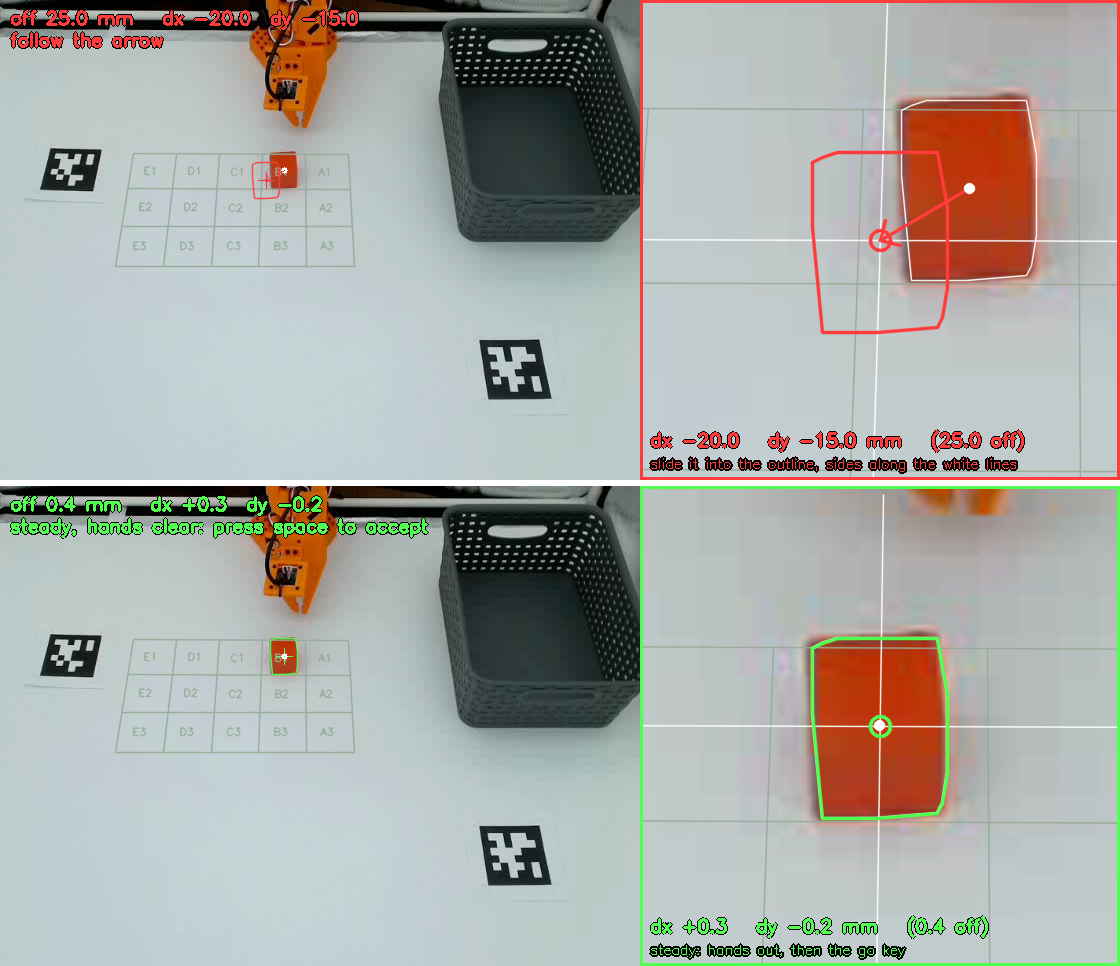
\includegraphics[width=0.82\textwidth]{figures/fig5-overlay-example.png}
\caption{The placement overlay as the operator sees it, rendered afterwards with the session's own code from the first frame of a counted trial's video. Left: the front camera's image with the grid (which is not marked on the floor) and its cell names, the two floor tags, the arm at its start pose and the basket. Right: the surroundings of the target, magnified. Top: the cube 25~mm from a target chosen for this illustration; the outline shows where the cube belongs, and the readout gives the offset in table millimetres. Bottom: the same frame against the trial's own target, within tolerance (0.4~mm from it).} % src: scripts/make_overlay_example.py and its output of 2026-10-09 (trial T1a-001: 25.0 mm from the shown target, 0.4 mm from the planned one)
\label{fig:overlay}
\end{figure*}

\emph{The table frame: tags, grid and registration.}
The grid is virtual: nothing is drawn on the floor, so that the policy sees no marks of position. The cameras see only the floor, two fiducial tags and the basket, and the grid appears in the overlay alone (Fig.~\ref{fig:overlay}). % src: protocol/protocol.md, section 3 ("The grid ... is virtual: nothing is drawn on the floor"); the reason as the operator gave it on 2026-10-09 (docs/journal.md): no record of the design days states it
Two AprilTags (Table~\ref{tab:rig}) are taped to the floor outside the grid, one in front on the right of the arm and one at the rear on the left, and tie the grid to the floor. % src: docs/runbook/00-table-layout.md, step 1 (tag 0 front right, tag 1 rear left)
Their positions in the grid's frame were measured once, in a \emph{registration}: a printed sheet carrying the grid's outline and six 36~mm tags was laid where the grid should be, the conversion from pixels to table millimetres was fitted through the six tags over 40 frames, the corners of the two floor tags were stored in that frame, and the sheet was removed. % src: config/table_geometry.json, registration (method, sheet_tags, frames); protocol/protocol.md, section 7
Two findings from the first evening shaped this design. First, a frame solved from the two floor tags alone is fragile: one pixel on one tag corner moves the far side of the grid by up to 2.5~mm, so the two tags are used to carry a frame that six tags established, and not to establish it. % src: analysis/instrument/first_sitting.md, section 3 (2.51 mm); protocol/protocol.md, section 7 ("a watchman, not a ruler")
Second, the tag detector's corners lie about 0.6 pixels inside a tag's outline at this view (about one pixel per millimetre) and move with the image's brightness, so every tag is measured by lines fitted to its outline instead. % src: config/table_geometry.json, registration.detector_inset_px (0.56); analysis/instrument/first_sitting.md (0.61 px); protocol/protocol.md, section 7
Because the camera hangs from the light box's frame, which the box's walls move (closing one zipper turned the camera by 0.1 degrees), each session solves the conversion again from the two floor tags as it finds them. % src: protocol/protocol.md, section 7 ("every session solves it afresh"); docs/runbook/00-table-layout.md, step 2 (the zipper, 0.1 degrees)

\emph{How the frame performed.}
At the registration, the six sheet tags fitted one plane to 0.41~mm on average (0.88~mm at most); a tag left out of the fit was predicted by the other five to 0.61~mm on average (1.91~mm at most); and the sheet's printed grid lines, which no fit uses, lay 0.28~mm (root mean square) from the fitted frame. % src: config/table_geometry.json, registration: sheet_fit_mean_mm 0.41, sheet_fit_max_mm 0.876, leave_one_out_mean_mm 0.613, leave_one_out_max_mm 1.914, sheet_lines.rms_mm 0.284
In use, the checks reported in Section~\ref{sec:instrument} and Table~\ref{tab:rigb} apply: steps of 10~mm were read to \instrumentMeanAbsError~mm on average, repeated readings of one position stayed within \repeatabilityScatter~mm, and accepted placements were a median of \resetErrorMedian~mm from their targets. % src: protocol/protocol.md, section 7 (the step of the scale check)
The weak point was the camera's mounting, not the tags: at the start of the six sessions with counted trials the camera's image stood 0.4 to 1.7~mm from the stored calibration, the two floor tags read 1.6 to 1.8~mm against each other relative to the registration (the rest of the image had moved with them, which indicates a rotation of the camera and not a tag's movement), and two sessions ended on the rule that allows no attempt once the image has moved more than \viewCreptLimit~mm within a session. % src: docs/decisions.md, 2026-10-08 (the six counted sessions' kept start frames read again on 2026-10-08: the camera 0.37 to 1.70 mm; the tags 1.6, 1.7, 1.8, 1.8, 1.7 and 1.8 mm, said beyond 1.5 and refused beyond 3); protocol/protocol.md, section 7 (the tags' reading follows the camera's turn); docs/journal.md, 2026-10-08 (the sessions of 13:21 and 15:38 ended by the creep rule)
A camera mount that is independent of the enclosure would remove that cost.

\emph{The instrument.}
The front camera detects the cube and converts its position to table millimetres. Each session solves this conversion from the outlines of the two floor tags, averaged over 20 frames, and measures through it; the start position of a demonstration is measured through the tags as that episode's first frame shows them. % src: protocol/protocol.md, section 7 ("The frame is the floor tags', and every session solves it afresh")
A calibration stored once serves as a reference only: a session reports a difference above 1.5~mm from it and stops above 5~mm. % src: protocol/protocol.md, section 7
The detector reports the centre of the cube's visible outline (its top and lit sides) mapped through the table plane, not the centre of its footprint.
The same holds for every demonstration and every trial, so the offset cancels in a distance, but only up to a scale factor, which geometry places a few percent above one.
Over its \nScaleRuns runs the scale check gave a factor, each run's measured length divided by its true length (50 to 150~mm), between \scaleFactorMin and \scaleFactorMax (mean \scaleFactor). % src: analysis/report/report.md, "Scale check" (runs of 60, 50, 150 and 50 mm)
The rule fixed in advance: if the runs agree within one percentage point, every distance in the analysis is divided by the mean factor; otherwise, distances are left as measured and the range of the factor is reported as the instrument's accuracy.
A placement (Fig.~\ref{fig:overlay}) is accepted when the cube is steady within \placementTolerance~mm of its target and the operator, with hands out of the camera's view, presses a key; only then can the arm move, and the position at that moment is the measured start.
For repeatability, the cube was pushed \nRepeatability times against a fixed stop and lifted away between readings; the readings stayed within \repeatabilityScatter~mm of their mean.
No overlay was involved, so this figure describes the detector alone. % src: protocol/protocol.md, section 7, item 2 ("A stop, not the overlay"); data/instrument/repeat_20261008_174537.csv

\emph{Resets by eye.}
For each of \nByEye targets, the cube was returned to its position using a reference image shown beside the live view, with no overlay and no readout.
Number of people who placed the cube by eye: \nOperatorsByEye; the largest error was \byEyeErrorMax~mm.
This corresponds to an evaluation that resets the object ``to the same place'' from an image or from memory.
It does not correspond to an evaluation that overlays a reference image on the live view; we did not measure that case and expect its error to lie between that of resets by eye and that of the resets of this study.

\emph{Recording.}
One operator recorded both sets on one day with the same task text, time limit, cube orientation (square to the grid), start pose, approach side and grasp, in rounds of one episode per trained cell in shuffled order; an episode ended when the operator pressed a key, so episodes differ in length (Table~\ref{tab:rigb}). % as recorded: data/recording/*_placements.jsonl (ten rounds of 11 episodes, 11 distinct trained cells each, on 2026-10-07); data/audit/*_rate.json (17 to 26 s)
An episode was recorded again when the operator made a handling error, the cube was outside tolerance or a check failed.
The protocol plans a practice block that is recorded and discarded; the procedure of the recording day asks for practice without recording, and the logs hold no practice episode. % src: protocol/protocol.md, section 4 ("A practice block of about 10 episodes is recorded first and discarded"); docs/runbook/02-arm-and-recording.md, step 4 (practice, nothing recorded); data/recording/*_placements.jsonl
The clustered layout repeats each location to within about a millimetre: the \nDemosPerCell start positions at a location are within \clusteredScatterMax~mm of their mean.
In our earlier dataset, where the cube was placed using a grid drawn over the camera image and the start positions were not measured, the two farthest of a cell's five demonstrations were 4.8 to 13.7~mm apart, so a location repeated without a measuring aid is itself somewhat spread. % src: protocol/protocol.md, section 4 ("This clustered set is tighter than August's"); analysis/pilot_august/README.md (4.8 mm in cell A3 to 13.7 mm in cell D1, through one conversion)
The two layouts compared here are therefore the two extremes of a range; a recording made without a placement aid lies between them.
Before training, each dataset was checked for its episode and frame counts, the decoding of both camera streams, frame pacing and torn frames (Appendix~\ref{app:faults} reports the results of the last two), and by the start-state audit: every episode in its planned cell and within 3~mm of its target. % src: protocol/protocol.md, section 4 (dataset checks before training)

% ======================================================================================================================
\section{The protocol: predictions, analysis and stop rules}
\label{app:protocol}
The protocol (version \protocolVersion) was frozen before the first counted trial. % src: config/protocol.toml (version 1.0, status frozen); git tag protocol-v1, 2026-10-08 12:50:13; the first counted trial began at 13:22:47
A \emph{counted} trial is one run under the frozen protocol, and only counted trials are analysed.
Before the freeze, \emph{pilot} trials tested the procedure: a replay pilot, and nine exact repeats with the clustered policy (the second stop rule below). % src: protocol/protocol.md, sections 8 and 12
Pilot trials were written to separate logs, and the trial runner does not start a counted trial until the protocol is frozen.
The predictions below were written three days before the first counted trial and two before the first pilot trial, and were not changed after the day they were written. % src: git history of protocol/protocol.md: section 9 at tag protocol-v1 is word for word that of commit ce89dba (2026-10-05 20:53); the workspace test's placements, which prediction 3 is about, were last changed that evening too (draft 0.3, commit 8c22c0a, 22:58); the first pilot trial is of 2026-10-07 17:24 (data/trials/pilot_shakedown.jsonl)

\subsection{Predictions stated before the data}
Every radius in this list is a block fit (defined below).
\begin{enumerate}
\item \emph{The curve.} The clustered policy succeeds at least 5 times in \anchorsZeroClustered at $d=0$ and at most once in \anchorsFarClustered at \farLevel~mm, and its radius lies between 5 and 40~mm. % src: protocol/protocol.md, section 9, prediction 1
\emph{Observed:} \successZeroClustered of \nZeroClustered, \successFarClustered of \nFarClustered, and \radiusClusteredThreshold~mm (\radiusClusteredThresholdLow to \radiusClusteredThresholdHigh). Only the median met the prediction: the interval extends to \radiusClusteredThresholdHigh~mm, and the median of the second fit of the plateau check, \radiusClusteredThresholdWide~mm, lies outside the predicted range (Table~\ref{tab:plateau}).
\item \emph{Hardware.} The policy's radius is larger than the replay's, by the rule for ``larger'' below.
\emph{Observed:} a difference of \radiusDiffClusteredReplay~mm (\radiusDiffClusteredReplayLow to \radiusDiffClusteredReplayHigh), and a posterior probability $\probClusteredExceedsReplay$ that the policy's radius is the larger. The prediction was met under the pre-specified rule; the policy's radius itself is not established.
\item \emph{Layout.} At the placements of the workspace test, the spread policy succeeds more often than the clustered one. % src: protocol/protocol.md, section 9, prediction 3 (its wording; where the placements are drawn is in "The blocks as planned")
\emph{Observed:} \workspaceSuccessSpread against \workspaceSuccessClustered of \nPairs ($p=\mcnemarP$). The prediction was not met: the counts are in the predicted direction, but the test does not establish a difference.
\item \emph{Lookup.} Each policy's success in the workspace test matches the lookup prediction: its observed count lies inside the prediction's \intervalLevel~\% interval.
\emph{Observed:} \workspaceSuccessClustered against a predicted \lookupPredictedClustered (\lookupClusteredLow to \lookupClusteredHigh) for the clustered policy, and \workspaceSuccessSpread against \lookupPredictedSpread (\lookupSpreadLow to \lookupSpreadHigh) for the spread policy. The prediction was met, with wide intervals and conditional on the curve from which it is computed.
\item \emph{Layout and radius.} No prediction; reported as an estimate.
\emph{Observed:} not available. The spread policy's threshold block was not run (Appendix~\ref{app:counts}), so it has no block fit and the two radii are not compared; its workspace-test trials alone bound its radius from below, at \radiusSpreadLow~mm.
\end{enumerate}

\subsection{The blocks as planned}
Table~\ref{tab:design} gives each block.
Staircases move in steps of \stepInitial~mm until their first reversal and \stepFinal~mm after it, between 0~mm and the block's largest distance; the replay's may request up to \maxLevelReplay~mm. % src: config/protocol.toml, staircase.min_level_mm
A requested distance is met when the target's distance to its nearest demonstration is within \levelMatch~mm of it, and test placements keep the cube's centre at least \testMargin~mm inside the grid's edge.
For a replay the target is drawn uniformly in direction on the circle of that radius around the start of the demonstration played back.
The held-out cells are \heldOutCells.
Inside a trained cell no point is farther than about \clusteredMaxDistInCell~mm from a clustered demonstration, or than about 17~mm from a spread one; larger distances are tested in held-out cells. % src: protocol/protocol.md, section 4 (largest gap of the planned spread layout: 17.2 mm; of the clustered one: 35.4 mm)
The far anchor trials are set at \farLevel~mm and not at \maxLevelClustered~mm, where nearly every admissible point lies in a corner cell; at \farLevel~mm the two interior held-out cells also contain admissible points.
The workspace test draws \nPairsTrainedPlanned of its \nPairsPlanned placements uniformly over the trained cells and \nPairsHeldOutPlanned over the held-out cells, and tests them in one shuffled order.
With placements in trained cells only, the paired test could detect no difference once the radius is large enough for the clusters to cover their own cells; with placements in held-out cells only, it could detect none while the radius is small. A calculation under the lookup model, made before any trial, was used to choose the design. % src: protocol/protocol.md, section 8, and analysis/simulation/workspace_designs.md (the designs compared, and how often each would reach p < 0.05)
Both policies were to be evaluated at step \trainSteps; had a run not reached it in time, both would have been evaluated at their largest common saved step, and not below \trainStepsFallback.

\emph{The replay.}
The replay block plays back \nReplayDemosPlanned demonstrations of the clustered set, one from each trained cell, so that the replay is tested over the same regions of the table as the policy; the planner's seed draws which of a cell's \nDemosPerCell it is, before any trial.
The block's \plannedReplay trials replay each demonstration twice, in two different parts of the block: the \anchorsZeroReplay trials at $d=0$ are \anchorsZeroReplay different demonstrations, and each staircase replays \stairTrialsReplay different ones. % src: protocol/protocol.md, section 6 ("twice" holds because the block has two trials for each demonstration; a test of config/protocol.toml holds it to that)
Which demonstration a trial replays does not depend on any outcome.
In the replay pilot, each of the \nReplayDemosPlanned demonstrations was replayed once from its own start position: ten succeeded, and the eleventh attempt was terminated by an accidental key press and is logged as a failure. % src: data/trials/pilot_replay.jsonl (the 11 trials at level 0: 10 successes; T1b-022, note "accidental keyboard type", 5.7 s); protocol/protocol.md, section 6 asks for this count
The safety gate that transfers control of the motors allows a replay to begin only when every joint is within \handoffToleranceReplay degrees of that demonstration's first recorded action, so a replay starts from approximately the pose from which the demonstration started.
A policy trial has a looser tolerance of \handoffTolerance degrees: the policy observes the arm and may start from any nearby pose.

\emph{Order and blinding.}
The trials of the clustered policy's block and of the replay block, \plannedClustered and \plannedReplay, are shuffled into one seeded order, so that the policy and the replay are tested at the same time of day, at the same servo temperature and in the same state of the cameras.
The workspace test follows, with the two trials of a pair in immediate succession on the same target and each policy first in half of the pairs; the spread policy's block was planned last and was not run.
As run, the interleaved order took four consecutive sessions in about 91 minutes: one session was ended by the rule on camera movement (Table~\ref{tab:rigb}) and two after the arm had displaced the basket (see below). The workspace test followed 47 minutes later, in two sessions, the first of which was ended by the same rule; no pair was split between sessions. % src: data/trials/main.jsonl (ts_start, media folders, notes); docs/journal.md, 2026-10-08
A trial is identified to the operator by a running number and a code drawn from one shuffled list.
Neither indicates which policy runs, which block the trial belongs to, or whether it is a replay.

\emph{The second scoring.}
Every attempt was recorded on video by both cameras.
After the last trial, one scored trial in five of each condition of each block (\nSecondScored of \nTrialsTotal) was drawn by a seed and the hash of the trial log itself, so that it could not be known in advance which trials would be scored again; the two trials of a workspace pair were never both drawn. % src: protocol/protocol.md, section 8 ("A second scoring from video")
These trials were scored again from the videos alone, under neutral names and in shuffled order, with no condition, distance or first score shown.
No second person was available, so the operator who had scored at the rig gave both scores.
The two scores agree in \nSecondScoredAgree of \nSecondScored trials; in \nSecondScoredCannotTell trials the video did not show the outcome.
The score given at the rig remains the trial's outcome regardless of the second score.

\emph{Void trials and failures.}
A trial is void when it could not test its condition: the placement was later found outside tolerance, a camera or motor fault ended the attempt, a person interfered, the safety gate refused the start three times, or a key press ended the attempt within one second of its start.
A void trial remains in the log with its reason, and its position in the plan is repeated with the same target, under a new number and a new code. % src: protocol/protocol.md, section 8 (the five reasons)
A stop caused by the condition's own motion after the handover (the per-step clamp, the stall rule) is a failure.

\emph{The basket and the wrist camera.}
The basket is fixed to the floor with double-sided tape. At a release, the wrist camera's mount can strike the basket's rim and displace it, and the same contact can shift that camera in its mount.
A trial in which this happens keeps its score; the basket is then repositioned with a live overlay of a reference image, and the wrist camera's position is read from the position of the gripper's fixed jaw in its image.
The first frames of each trial's own videos were read afterwards. The arm displaced the basket by more than 5~mm in \nTrialsBasketMoved trials (by 35 and 45~mm). In \nTrialsBasketNamed trials the basket began more than 2~mm from its reference position, in all of them between 2.1 and \basketStartMax~mm: one pixel is about 1.1~mm there, so these readings are two pixels from the reference. The number of trials that began with the jaw more than 2 pixels from its position in training was \nTrialsWristNamed (\wristStartMax pixels at most; the camera's view was offset by about 2 pixels before the first block and was not corrected). The analysis report lists the trials by identifier. % src: protocol/protocol.md, section 8 (the two limits); data/audit/scene_main.json (basket_moved_mm of the two trials; the start readings); src/tolerance_radius/rig/basket_place.py, MM_PER_PX (1.08); docs/decisions.md, 2026-10-08 (the wrist camera is left where it stands)

\begin{table}[t]
\caption{The blocks as planned. Distances in millimetres.}
\label{tab:design}
\centering
\footnotesize
\setlength{\tabcolsep}{4pt}
\begin{tabular}{@{}lcccc@{}}
\toprule
 & Trials & Trials at & Two staircases: & Largest \\
Block & at $d=0$ & \farLevel~mm & starts; trials each & distance \\
\midrule
Replay & \anchorsZeroReplay{} & -- & \stairStartNearReplay{} and \stairStartFarReplay{}; \stairTrialsReplay{} & \maxLevelReplay{} \\
Clustered policy & \anchorsZeroClustered{} & \anchorsFarClustered{} & \stairStartNearClustered{} and \stairStartFarClustered{}; \stairTrialsClustered{} & \maxLevelClustered{} \\
Spread policy & \anchorsZeroSpread{} & -- & \stairStartNearSpread{} and \stairStartFarSpread{}; \stairTrialsSpread{} & \maxLevelSpread{} \\
Workspace test & \multicolumn{4}{l}{\nPairsPlanned placements, each with both policies:} \\
 & \multicolumn{4}{l}{\nPairsTrainedPlanned in trained cells, \nPairsHeldOutPlanned in held-out cells} \\
\bottomrule
\end{tabular}
\end{table}

\subsection{Analysis fixed in advance}
\begin{itemize}
\item \emph{Model and estimate.} Eq.~\eqref{eq:model}, with a posterior on a grid: a flat prior on $r_{50}$ from 0 to \gridRadiusMax~mm in steps of 0.5~mm, a flat prior on $\log w$ over 30 values from \gridWidthMin to \gridWidthMax~mm, and $\lambda\in\{\lapseValues\}$ and $\gamma\in\{\floorValues\}$, the values of each equally weighted. % src: config/protocol.toml, analysis.r50_grid_mm (min, step) and analysis.width_grid_mm.count
We report the posterior median of $r_{50}$ and its equal-tailed \intervalLevel~\% interval.
The staircases only choose where to test.
\item \emph{Rationale for the floor.} A trial far from every demonstration can still succeed by chance.
In the earlier evaluation one did, through a grasp at the cube's edge at 40~mm, and with the floor fixed at zero that single trial changed the fitted radius from 19.5 to 26~mm. % src: analysis/pilot_august/README.md, "Where the 50 % point can be" (the model of protocol draft 0.1, without a floor; trial 28)
The floor values limit the influence of such a success on the radius.
They do not measure how often chance successes occur; the far anchor trials give that as a count.
\item \emph{An interval that is open on a side.} The interval is \emph{open} on a side when the posterior at that end of the grid is at least half of what it is at the interval's own bound on that side.
We then report ``at most'' the upper bound (open below) or ``at least'' the lower bound (open above), and not a radius.
This occurs when success is already decreasing at $d=0$, or is still on its plateau at the largest distance tested.
\item \emph{The plateau is checked.} The lapse values above stop at 0.10, which suits a condition that nearly always succeeds at a demonstration's own start. % src: config/protocol.toml, analysis.lapse_values (the largest)
With a lower plateau the model would account for failures near a demonstration by a smaller radius: in simulation, a true plateau of 0.65 reduced the estimated radius by 8~mm. % src: protocol/protocol.md, section 10 (analysis/simulation/lapse_values.md); simulated, not measured
Every fit is therefore made a second time with $\lambda\in\{\lapseValuesWide\}$, and both fits are reported with the counts at $d=0$ (Table~\ref{tab:plateau}).
The first fit gives the radius we report. If the two medians differ by more than \plateauShiftLimit~mm, we state that the condition's plateau is uncertain and its radius not established, and every result that depends on that radius (a comparison, the lookup prediction, the reset sensitivity, prediction 1) is still computed by its rule and reported with that caveat. % src: protocol/protocol.md, section 10 (what rests on a radius; "prediction 1" is the first item of the list above)
Here the clustered policy's pooled fit changed by \plateauShiftClustered~mm, so the caveat applies to this policy; its block fit changed by \plateauShiftClusteredThreshold~mm.
Over all 60 of its scored trials, the policy succeeded in all 11 trials within 10~mm of a demonstration, in 6 of 10 between 10 and 20~mm, and in 9 of 12 between 30 and 40~mm (all of the latter in held-out cells): the decline is gradual and location matters besides distance (Section~\ref{sec:results}), which a single curve of distance does not represent. % src: analysis/report/report.md, "Clustered policy", the table of 10 mm bins over its 60 scored trials
\item \emph{Two fits.} The \emph{block fit} uses a condition's own threshold block only.
Every comparison and every prediction uses block fits: the comparison of the policy with the replay, two blocks of one session, and the lookup prediction, which must not have seen the workspace-test trials it predicts.
The \emph{pooled fit} adds a policy's workspace-test trials at their measured distances, and is reported alongside the block fit as a check that the two agree.
The spread policy's threshold block was not run, so it has a pooled fit only, from its workspace-test trials: placements fixed in advance and not chosen by a staircase, half of them in held-out cells.
\item \emph{The radius as the reported quantity.} We report $r_{50}$ and not $w$: thresholds need far fewer trials than slopes \cite{kontsevich1999bayesian}, and slopes fitted to adaptive data are biased \cite{kaernbach2001slope}.
\item \emph{Without a model.} Success counts in 10~mm bins of $d$, closed below and open above, with Wilson intervals \cite{wilson1927probable}; the largest $d$ with a success and the smallest with a failure. % src: protocol/protocol.md, section 10
\item \emph{Comparison of radii.} The posterior probability that one condition's $r_{50}$ exceeds another's, from the two block fits taken as independent, and the difference with its interval.
``Larger'' means a probability of at least 0.95 and ``smaller'' one of at most 0.05; anything between is reported as not distinguished by these trials. % src: protocol/protocol.md, section 9, prediction 2
\item \emph{Workspace test.} The table of paired outcomes, the exact McNemar test, and each policy's success with a Wilson interval.
All placements make one test; the counts for trained and for held-out cells apart, a pair counting by the cell its cube was measured in, are descriptive.
We call the two policies different at these placements when the test's two-sided $p$ is below 0.05, the level at which we state below what the test can show. % src: protocol/protocol.md, section 9, prediction 3 (the rule: the exact paired test, p below 0.05) and section 8
\item \emph{Lookup prediction.} For each placement and policy, the predicted probability of success is the clustered policy's block fit at that placement's measured distance to the policy's own nearest demonstration, averaged over the posterior.
We report the expected number of successes, the \intervalLevel~\% interval of the predicted count, which carries both the uncertainty of the fit and the chance in \nPairsPlanned trials, the observed count, and whether it lies inside.
The fit comes from a block run earlier in the day, so a change in the rig between the two would also appear as a mismatch.
\item \emph{Reset sensitivity.} The success the clustered policy's block fit gives at trained positions if resets carry the by-eye errors, beside the same calculation with this study's own placement errors. A calculation, not a measurement.
The curve is evaluated at a distance equal to each of the \nByEye by-eye errors, and to each of the \nTrialsTotal placement errors of the scored trials, and the results are averaged. The result: \resetSensitivityByEye~\% with the by-eye errors against \resetSensitivityPlaced~\% with this study's placement errors, conditional on a fitted curve whose radius is not established; it does not apply to resets made with an overlay.
\item \emph{Descriptive only.} Success by placement inside or outside the convex hull of the demonstrations; failure labels by distance; durations; the achieved control rate.
\item \emph{Exclusions.} No trial is excluded except void trials and pilot trials, and no outcome is changed after the fact.
\end{itemize}

\begin{table}[t]
\caption{The plateau check: each fit made with the lapse values of the analysis (up to 0.10) and again with the longer list (up to 0.50). Posterior median and \intervalLevel~\% interval of $r_{50}$ in millimetres; an interval that the data do not bound above is given as its lower bound, and the median of such a fit is shown only to give the shift, which is the second median minus the first. The second column gives the successes at $d=0$ among the fit's trials.} % src: config/protocol.toml, analysis.lapse_values and analysis.lapse_values_sensitivity (their largest values)
\label{tab:plateau}
\centering
\footnotesize
\setlength{\tabcolsep}{1.8pt}
\begin{tabular}{@{}lcccccc@{}}
\toprule
 & At & \multicolumn{2}{c}{$\lambda\le 0.10$} & \multicolumn{2}{c}{$\lambda\le 0.50$} & \\ % src: the same two lists
Fit & $d=0$ & median & interval & median & interval & Shift \\
\midrule
Replay, block & \successZeroReplay{}/\nZeroReplay{} & \radiusReplay{} & \radiusReplayLow{}--\radiusReplayHigh{} & \radiusReplayWide{} & \radiusReplayWideLow{}--\radiusReplayWideHigh{} & \plateauShiftReplay{} \\
Clustered, block & \successZeroClustered{}/\nZeroClustered{} & \radiusClusteredThreshold{} & \radiusClusteredThresholdLow{}--\radiusClusteredThresholdHigh{} & \radiusClusteredThresholdWide{} & $\geq$\,\radiusClusteredThresholdWideLow{} & \plateauShiftClusteredThreshold{} \\
Clustered, pooled & \successZeroClustered{}/\nZeroClustered{} & \radiusClustered{} & \radiusClusteredLow{}--\radiusClusteredHigh{} & \radiusClusteredWide{} & \radiusClusteredWideLow{}--\radiusClusteredWideHigh{} & \plateauShiftClustered{} \\
Spread, pooled & none & \radiusSpread{} & $\geq$\,\radiusSpreadLow{} & \radiusSpreadWide{} & $\geq$\,\radiusSpreadWideLow{} & \plateauShiftSpread{} \\
\bottomrule
\end{tabular}
\end{table}

\subsection{What the trial budget can show}
Before the freeze we simulated each threshold block against success curves assumed true and fitted it as the analysis fits the real trials (\simReplications simulated blocks for each curve).
Every figure in this subsection is simulated or computed from stated assumptions; none is a measurement.

\emph{One radius.}
For the clustered policy's block and an assumed curve with $r_{50}=\simTruthRadius$~mm and $w=\simTruthWidth$~mm, the estimated radius differed from the true radius by \simBias~mm on average, with a root-mean-square error of \simRmse~mm; its interval was \simIntervalWidth~mm wide on average and held the true radius in \simCoverage~\% of blocks.
The same number of trials at fixed, equally spaced distances gave an error of \simRmseConstant~mm and an interval \simIntervalWidthConstant~mm wide, which is why the staircases were kept.
The precision depends on how steep the true curve is, which is not known before the trials: Table~\ref{tab:simblocks} gives each threshold block's simulated error and interval width for a steep curve ($w=\simWidthCliff$~mm), an intermediate one ($w=\simWidthMiddling$~mm) and a shallow one ($w=\simWidthSlope$~mm).
Where success is already decreasing at $d=0$, the interval was open below in \simOpenBelow~\% of simulated blocks: the estimate is then reported as ``at most'' and not as a radius.
\begin{table}[h]
\caption{Simulated before any trial: root-mean-square error of the estimated radius / mean width of its \intervalLevel~\% interval, in millimetres, for each threshold block as planned and three widths of the assumed curve. These values are simulated, not measured.}
\label{tab:simblocks}
\centering
\footnotesize
\begin{tabular}{@{}lccc@{}}
\toprule
Block & Steep & Intermediate & Shallow \\
\midrule
Clustered policy & \simRmseClusteredCliff{} / \simIntervalWidthClusteredCliff{} & \simRmseClusteredMiddling{} / \simIntervalWidthClusteredMiddling{} & \simRmseClusteredSlope{} / \simIntervalWidthClusteredSlope{} \\
Replay & \simRmseReplayCliff{} / \simIntervalWidthReplayCliff{} & \simRmseReplayMiddling{} / \simIntervalWidthReplayMiddling{} & \simRmseReplaySlope{} / \simIntervalWidthReplaySlope{} \\
Spread policy & \simRmseSpreadCliff{} / \simIntervalWidthSpreadCliff{} & \simRmseSpreadMiddling{} / \simIntervalWidthSpreadMiddling{} & \simRmseSpreadSlope{} / \simIntervalWidthSpreadSlope{} \\
\bottomrule
\end{tabular}
\end{table}

\emph{Two radii.}
How large a difference between the policy's radius and the replay's radius the rule for ``larger'' can detect depends on how steep the two curves are, and the rule can also err when the two radii are equal.
Table~\ref{tab:simrule} gives, for a replay radius of \simRuleReplayRadius~mm and \simRulePairs simulated pairs of blocks per case, how often the rule returned ``larger''.
At equal radii it returned ``larger'' in \simRuleLargerWidthThreeDiffEqual~\% of pairs and ``smaller'' in \simRuleSmallerWidthThreeDiffEqual~\% (both curves of width \simWidthMiddling~mm).
\begin{table}[h]
\caption{Simulated before any trial: share of pairs of blocks (clustered policy, replay) in which the rule returned that the policy's radius is the larger, in percent, by the true difference of the two radii and the width of both curves. These values are simulated, not measured.}
\label{tab:simrule}
\centering
\footnotesize
\setlength{\tabcolsep}{4pt}
\begin{tabular}{@{}lcccccc@{}}
\toprule
Width & equal & +3~mm & +5~mm & +8~mm & +10~mm & +15~mm \\ % src: analysis/simulation/comparison_rule.md, the cases simulated
\midrule
1~mm & \simRuleLargerWidthOneDiffEqual & \simRuleLargerWidthOneDiffThree & \simRuleLargerWidthOneDiffFive & \simRuleLargerWidthOneDiffEight & \simRuleLargerWidthOneDiffTen & \simRuleLargerWidthOneDiffFifteen \\ % src: analysis/simulation/comparison_rule.md, the cases simulated
3~mm & \simRuleLargerWidthThreeDiffEqual & \simRuleLargerWidthThreeDiffThree & \simRuleLargerWidthThreeDiffFive & \simRuleLargerWidthThreeDiffEight & \simRuleLargerWidthThreeDiffTen & \simRuleLargerWidthThreeDiffFifteen \\ % src: analysis/simulation/comparison_rule.md, the cases simulated
6~mm & \simRuleLargerWidthSixDiffEqual & \simRuleLargerWidthSixDiffThree & \simRuleLargerWidthSixDiffFive & \simRuleLargerWidthSixDiffEight & \simRuleLargerWidthSixDiffTen & \simRuleLargerWidthSixDiffFifteen \\ % src: analysis/simulation/comparison_rule.md, the cases simulated
\bottomrule
\end{tabular}
\end{table} % src: analysis/simulation/comparison_rule.md; the column heads are that report's cases

\emph{Two policies at the same placements.}
With \nPairsPlanned pairs and true success rates of \simPairedRateLow and \simPairedRateHigh~\%, the exact McNemar test reaches $p<0.05$ in \simPairedPower~\% of cases, by an exact sum that takes the two outcomes at a placement as independent. % src: the level the procedure simulation uses for its power table
It cannot reach that level with fewer than six discordant pairs, and with six only if all six favour the same policy. % src: arithmetic, two-sided exact test: 2 x 0.5^6 = 0.031, and 2 x 0.5^5 = 0.0625
The test therefore detects only large differences; where the two policies are closer, we can report only the counts and their intervals.

\subsection{Stop rules}
Table~\ref{tab:stops} gives the criteria fixed in advance.
What happened at each is as follows.
\emph{Before recording:} the scale check passed (Section~\ref{sec:instrument}) and the camera's reference was stored. The rig check passed its five steps on the arm and the cameras and failed its last step, a comparison of the front camera's image with a stored one, on a stream that had opened without the manually set exposure; the image matched the stored one again a minute later. No complete pass of that check was recorded afterwards, and the rule for a missed line (omit the spread set) was not applied: both sets were recorded the next day. From then on every session, and the recorder at every episode, compared the image's white and black levels with those of the stored calibration before proceeding. This happened two days before the protocol was frozen, so it is reported here and is not among the deviations from the frozen protocol. % src: docs/journal.md, 2026-10-06 (the rig check's sixth step, and the frame a minute later); analysis/report/report.md, "Scale check"
\emph{After recording:} both datasets passed their audits, and the pilot gave 8 successes in 9 exact repeats (trials at a demonstration's own start), the minimum required. % src: data/audit/clustered.json and spread.json; data/trials/pilot_policy.jsonl (9 scored trials at 0 mm, 8 successes)
\emph{During the trials:} the two interleaved blocks were complete at 14:54, before the set time of 15:00. % src: data/trials/main.jsonl (the last trial of blocks T1a and T1b); protocol/protocol.md, section 12
\emph{End of the trials:} those two blocks and the workspace test were complete. The spread policy's block was then omitted by a decision of the operator and not under the third criterion; it is the first deviation listed in Appendix~\ref{app:counts}. % src: docs/decisions.md and docs/journal.md, 2026-10-08

\begin{table}[t]
\caption{Stop rules fixed before the experiment.}
\label{tab:stops}
\centering
\footnotesize
\begin{tabular}{@{}p{0.16\columnwidth}p{0.39\columnwidth}p{0.32\columnwidth}@{}}
\toprule
When & Pass criterion & If missed \\
\midrule
Before recording & Rig check passes; camera baseline stored; scale check within 1.5~mm mean absolute error, no step deviating by more than 3~mm & Repair before recording; if that is not possible in time, omit the spread set \\ % src: protocol/protocol.md, sections 7 and 12
After recording & Both datasets recorded and audited; in a pilot, a clustered checkpoint succeeds in at least 8 of 9 exact repeats & Stop: no submission \\ % src: protocol/protocol.md, section 12
During the trials & The clustered policy's block and the replay block complete by a set hour & Skip the spread policy's block; run the workspace test only if all its pairs fit \\
End of the trials & The clustered policy's block and the replay block complete & Report the completed blocks, and state what was planned and not run \\
\bottomrule
\end{tabular}
\end{table}

% ======================================================================================================================
\section{Deviations, trial counts and void trials}
\label{app:counts}
The decision log records \nDeviations deviations from the frozen protocol. % src: docs/decisions.md, the three rows of 2026-10-08 marked as deviations; protocol/protocol.md, section 13
First, the spread policy's threshold block (\plannedSpread trials) was planned and not run. The protocol's rule for omitting it applies when the two interleaved blocks are not complete by a set time, and they were; the operator omitted it on the day of the trials, to allocate the remaining time to the by-eye resets, the repeatability check and the second scoring. At that point the operator had scored every trial without knowing its condition, and no count by condition had been computed. As a consequence the spread policy has no threshold block, and the two policies' radii are not compared. % src: protocol/protocol.md, sections 8 and 12; docs/decisions.md and docs/journal.md, 2026-10-08
Second, the repeatability check, which the protocol places before any trial, was run after the last trial on the same day.
Third, the check of the camera against the floor tags that the protocol places at the end of each block was not run as a separate step: the start of the next session, about 47 and 39 minutes after the last trial of the two blocks, made the same check, and both passed (0.8 and 0.7~mm from the stored calibration, where a session stops above 5~mm). % src: docs/decisions.md, 2026-10-08 (the two sessions' kept start frames, read again: 0.82 and 0.71 mm)
The second and third do not change what any trial measured.
Table~\ref{tab:counts} gives the trials planned, scored and void in each block.
Void trials: \voidReasons.
Of the descriptive results planned (Appendix~\ref{app:protocol}): every failure carries the label ``grasp'': 23 for the clustered policy (at 10.1 to 50.6~mm), 9 for the replay (14.7 to 25.4~mm) and 4 for the spread policy (16.1 to 38.3~mm). A trial's record lasted a median of 24~s, 24~s and 20~s, which is longer than the attempt itself. Inside the convex hull of its demonstrations the clustered policy succeeded in 28 of 36 trials and outside it in 9 of 24; the spread policy in 21 of 22 and 1 of 4. % src: analysis/report/report.md, "Descriptive only" (hull, failure labels with their ranges of d, median durations, in the order clustered policy, replay, spread policy)
Number of days on which trials ran: \nTrialDays. Number of people who placed the cube and scored: \nOperators.
Fig.~\ref{fig:workspace} shows the workspace test. In it both policies succeeded at \pairsBoth placements and neither at \pairsNeither; the placements were at most \workspaceDistClusteredMax~mm from a clustered demonstration and \workspaceDistSpreadMax~mm from a spread one.
The replay block played back \nReplayEpisodes demonstrations of the clustered set (planned: \nReplayDemosPlanned).

\begin{figure}[t]
\centering
\figureorbox{figures/fig4-workspace.pdf}{4.0cm}{The test placements on the grid, once per policy, with each policy's demonstrations, discs of the clustered policy's block-fit radius around them, and the outcome at each placement; predicted and observed counts below.}
\caption{The workspace test: each policy's demonstrations and the outcome at each of the \nPairs shared placements. In both panels the discs have the clustered policy's fitted radius $r_{50}$, which is not established; they are not a measured region of success. Below: successes and failures observed, and the successes the lookup prediction expects with its interval, for all placements and by kind of cell.}
\label{fig:workspace}
\end{figure}

\begin{table}[t]
\caption{Trials planned, scored and void, by block.}
\label{tab:counts}
\centering
\footnotesize
\begin{tabular}{@{}lccc@{}}
\toprule
Block & Planned & Scored & Void \\
\midrule
Replay & \plannedReplay{} & \nTrialsReplay{} & \nVoidReplay{} \\
Clustered policy, threshold & \plannedClustered{} & \nTrialsClusteredThreshold{} & \nVoidClusteredThreshold{} \\
Workspace test, both policies & \plannedWorkspace{} & \nTrialsWorkspace{} & \nVoidWorkspace{} \\
Spread policy, threshold & \plannedSpread{} & \nTrialsSpreadThreshold{} & \nVoidSpreadThreshold{} \\
\midrule
All & \plannedTotal{} & \nTrialsTotal{} & \nVoidTotal{} \\
\bottomrule
\end{tabular}
\end{table}

% ======================================================================================================================
\section{The earlier evaluation, re-analysed}
\label{app:earlier}
% Every number in this section is measured already. Each was recomputed on 2026-10-05 from
% analysis/pilot_august/trials_with_distance.csv, except where the line names analysis/pilot_august/README.md.
The earlier evaluation of Fig.~\ref{fig:earlier} tested one ACT policy on the same task, on this arm, with the front camera on a tripod instead of in the light box. % src: the earlier project's run journal (recording 2026-08-18 and all 31 trials on 2026-08-19 with the camera on a ground tripod; the light box from 2026-08-22). The same arm: one follower id and one calibration file, written 2026-07-03 and unchanged through this study (numbers_by_hand.tex, \rigCalibration)
Its 31 trials did not log the cube's start position. % src: trials_with_distance.csv, 31 rows
We measured it afterwards with the detector that had measured that policy's demonstrations: from the first frame of the trial's video in 30 trials, and from a still image saved at the start of the session for the one trial that was not recorded on video. % src: same file, position_source: 30 "video frame", 1 "session-start still"
The policy had been trained on 49 of the 55 demonstrations of its dataset, and distances are to the nearest of those 49. % src: analysis/pilot_august/README.md, "What was done", item 5 (read there from the earlier project's records)

The 19 trials in cells with demonstrations started 0.6 to 5.6~mm from the nearest trained demonstration, 17 of them within 3.1~mm, and all succeeded (Wilson 95~\% interval 83 to 100~\%). % src: same file, kind = id: d from 0.63 to 5.63; 17 rows at 3.03 or below; Wilson interval of 19/19 recomputed: 0.832 to 1
The 12 trials in held-out cells started 31 to 47~mm away and one succeeded, at 40~mm (1.5 to 35~\%). % src: same file, kind = ood: d from 31.01 to 47.14; the success is trial 28 at 40.01; Wilson interval of 1/12 recomputed: 0.015 to 0.354
With a second conversion from pixels to millimetres, one map for every image, the two groups are at 0.1 to 4.9~mm and at 32 to 47~mm: the untested range does not depend on the conversion. % src: same file, column d_nearest_trained49_mm_onemap: 0.11 to 4.89, and 32.46 to 46.89
In nine of the trials the cube had been placed on a demonstration's recorded start with an overlay that drew that demonstration's cube over the live view and showed the offset in pixels; those placements were 0.8 to 3.0~mm from it. % src: same file, ghost_error_mm in the 9 rows with a ghost_episode: 0.80 to 3.03

Three factors limit what that evaluation can show, in addition to the untested range.
Every near trial was in a cell with demonstrations and every far trial in a held-out cell, so it cannot separate distance from cell. % src: same file: all 19 rows with d below 10 have kind = id, all 12 above have kind = ood
The 31 trials are 12 scenes (a cell, or one demonstration's start re-created), each run two or three times, so they are not 31 independent tests and the intervals above are too narrow. % src: same file, scene_id: 12 distinct values, 2 or 3 rows each
Finally, the distances include a scale error that was not measured: the detector reads the centre of the cube's visible outline, not of its footprint, which, by geometry, makes measured distances a few percent too long. % src: analysis/pilot_august/README.md, "What these data cannot show" (an estimate from geometry, not a measurement)
The present study begins by measuring that scale.
% Not used, because it was not recomputed from the CSV (analysis/pilot_august/README.md, "How noisy the conversion is"):
% that evaluation's procedure gave its overlay tolerance of 4 pixels as "about 2 mm", and the re-analysis measured
% 4.2 to 5.3 mm. If the author verifies it, it is a direct example for the checklist's reset-accuracy entry.

% ======================================================================================================================
\section{Faults in the data pipeline of the earlier work}
\label{app:faults}
% THE COUNTS IN THIS SECTION ARE NOT IN THIS REPOSITORY. They are the \prior... macros of numbers_by_hand.tex, each copied
% from the earlier project's own records or measured again on its files; every line there says which (2026-10-08).
The earlier project's own records show three faults, each of which passes a check that the project had and each of which the project itself found within a day (Table~\ref{tab:faults}). % src: the earlier project's run journal, session logs, trial logs and git history, read on 2026-10-08; numbers_by_hand.tex has each line's source. There was no later audit: the project found each one at the time
We report them because each lies beneath the policy, in the data it is trained on or in how it is executed, and none would normally appear in a paper's method section.
We did not measure their effect on the policy.
None of three public dataset checkers lists, in its own description, a check of the decoded image for torn frames \cite{kunalsomani2026linted,jashshah2026lerobotdoctor,roboticsdata2026score}; this is a statement about what the descriptions list, not a test of the tools.
This study's own recording encountered torn frames again, and two further faults of the cameras; its records document them.
Two earlier attempts at the clustered set, recorded on the previous day, were not used: 4 episodes were discarded after the front camera's image changed in the middle of an episode, and 27 because the wrist camera had started with a different tone mapping of its image in 21 of them. % src: docs/decisions.md, 2026-10-06 and 2026-10-07 (the two rows that set the attempts aside)
In the two datasets that were used, a scan written for this rig (the earlier scan classified intact frames as torn on a white floor) flagged 9 frames in 6 of the 110 episodes; on individual inspection, 7 are torn, all in the top rows of the front camera's image, outside the area of the task. All episodes were kept and used for training. % src: docs/decisions.md, 2026-10-07 (the scan, and the pass line for torn frames); docs/journal.md of that day
No episode failed the pacing check, which here counts the control loop's cycles against wall-clock time rather than the nominal time stamps (Table~\ref{tab:rigb}). % src: data/audit/clustered_rate.json and spread_rate.json (fell_short is empty in both)

\begin{table*}[t]
\caption{Faults recorded in the earlier project's data and trials.}
\label{tab:faults}
\centering
\footnotesize
\begin{tabular}{@{}p{0.24\textwidth}p{0.24\textwidth}p{0.22\textwidth}p{0.20\textwidth}@{}}
\toprule
Fault & Extent & Checks that pass despite it & How it was found \\
\midrule
Torn video frames: one frame composed of parts of two frames & \priorTornFrames frames flagged in \priorTornEpisodes of the \priorDatasetEpisodes episodes behind the earlier evaluation & \priorTornChecks{} & \priorTornFound{} \\
Episodes captured more slowly than their time stamps say & \priorSlowEpisodes episodes at about \priorSlowRate~Hz, stamped 30~Hz & \priorSlowChecks{} & \priorSlowFound{} \\ % src: docs/reference/lerobot101-interfaces.md, section 2 (the stamped rate; confirm it against the earlier records)
An execution setting off without notice: \priorSettingOffName{} & \priorSettingOffTrials trials, kept apart from the reported ones & \priorSettingOffChecks{} & \priorSettingOffFound{} \\ % src: analysis/pilot_august/README.md, "Which video belongs to which trial line" (the lines were set aside)
\bottomrule
\end{tabular}
\end{table*}


\end{document}
